\documentclass{article}
\usepackage[a4paper]{geometry}
\usepackage{graphicx}
\usepackage{tikz}
\usepackage{dirtytalk}
\usepackage{pdfpages}
\usepackage{listings}
\usepackage[section]{placeins}
\usepackage{tocloft}
\usepackage[super]{nth}
\usepackage{lipsum}
\usepackage{wrapfig}
\renewcommand{\baselinestretch}{1.5}
\setlength{\parskip}{1em}
\usepackage{helvet}
\renewcommand{\familydefault}{\sfdefault}
\newcommand{\jump}[2]{\hyperlink{#1}{\colorlet{temp}{.}\color{black}{{\color{temp}#2}}\color{temp}}}
\usepackage[font=small,labelfont=bf]{caption}
\usepackage{lscape}
\usepackage{pdflscape}
\usepackage{array,tabularx}
\newenvironment{conditions*}
  {\par\vspace{\abovedisplayskip}\noindent
   \tabularx{\columnwidth}{>{$}l<{$} @{\ : } >{\raggedright\arraybackslash}X}}
  {\endtabularx\par\vspace{\belowdisplayskip}}
  
  \usepackage{scrlayer}
\usepackage{scrhack}
\DeclareNewLayer[
  background,
  textarea,
  addwidth=\footskip,
  addwidth=\footheight,
  contents=\hfill%
    \rotatebox{90}{\parbox{\layerheight}{\newgeometry{margin=4.7cm}\pagemark}}
]{lscape.foot}


\newcommand{\subsubsubsection}[1]{\paragraph{#1}\mbox{}\\}
\setcounter{secnumdepth}{4}
\setcounter{tocdepth}{4}
\usepackage{rotating}
\usepackage{abstract}
\renewcommand{\abstractnamefont}{\normalfont\large\bfseries}
\DeclareNewPageStyleByLayers{lscape}{lscape.foot}
\renewcommand{\cftsecleader}{\cftdotfill{\cftdotsep}}
\usepackage[sorting=none]{biblatex}
\addbibresource{bibliography.bib}
\usepackage{hyperref}
\usepackage{float}
\usepackage[nottoc, numbib]{tocbibind}
\graphicspath{ {./graphics/} }
\setlength\parindent{0pt}
\hypersetup{
    colorlinks,
    citecolor=black,
    filecolor=black,
    linkcolor=black,
    urlcolor=black
}

\begin{document}

%----------------------------------------------------------------------------------------
%	TITLE PAGE
%----------------------------------------------------------------------------------------

\begin{titlepage} % Suppresses displaying the page number on the title page and the subsequent page counts as page 1
	\newcommand{\HRule}{\rule{\linewidth}{0.5mm}} % Defines a new command for horizontal lines, change thickness here
	
	\center % Centre everything on the page
	
	%------------------------------------------------
	%	Headings
	%------------------------------------------------
	
	
    
\includegraphics[scale= 0.35]{img/logo.png}
    \bigskip
    
	\textsc{\LARGE Middlesex University}\\[1.5cm] % Main heading such as the name of your university/college
	
	\textsc{\Large School of Science and Technology}\\[0.5cm] % Major heading such as course name
	
	\textsc{\large CST3990 Undergraduate Individual Project}\\[0.5cm] % Minor heading such as course title
	
	%------------------------------------------------
	%	Title
	%------------------------------------------------
	
	\HRule\\[0.4cm]
	
	{\huge\bfseries eConsultant}\\[0.4cm] % Title of your document
	
	\HRule\\[1.5cm]
	
	%------------------------------------------------
	%	Author(s)
	%------------------------------------------------
	
	\begin{minipage}{0.4\textwidth}
		\begin{flushleft}
			\large
			\textit{Author}\\
			Marcel Kredzel\\ Student ID: M00540191
		\end{flushleft}
	\end{minipage}
	~
	\begin{minipage}{0.4\textwidth}
		\begin{flushright}
			\large
			\textit{Supervisor}\\
			Dr. David Gamez % Supervisor's name
		\end{flushright}
	\end{minipage}
	
	% If you don't want a supervisor, uncomment the two lines below and comment the code above
	%{\large\textit{Author}}\\
	%John \textsc{Smith} % Your name
	
	%------------------------------------------------
	%	Date
	%------------------------------------------------
	
	\vfill\vfill
	
	{\large April 30, 2021}
	
	\vfill
	
\end{titlepage}

%----------------------------------------------------------------------------------------
\begin{center}

\includegraphics[scale= 0.35]{img/logo.png}
    \bigskip
    
\textsc{\LARGE Middlesex University}\\[1.5cm] 

\textsc{\Large School of Science and Technology}\\[0.5cm]
\end{center}
{\large 
I hereby confirm that the work presented here in this report and in all other
associated material is wholly my own work.\par
}
\vfill\vfill
	\begin{minipage}{0.4\textwidth}
		\begin{flushleft}
			\large
			Signature:
			Marcel Kredzel\\ 
			Student ID: M00540191\\
			Date: April 30, 2021
		\end{flushleft}
	\end{minipage}
	~
	\begin{minipage}{0.4\textwidth}
		\begin{flushright}
		\end{flushright}
	\end{minipage}
	


\newpage
\begin{center}
    \section*{ABSTRACT}
\end{center}

{\large
There are various situations when a certain company has to make a crucial decision regarding their business and they choose to hire a consultant to help them in finding the best solution to the problem they are facing. Consultancy work is a complex process of analysing issues and solving them within a short space of time. Unfortunately, consultants cannot rely on any automation as there is not a single piece of software that could make their lives easier by analysing what has been said in meetings and what impact can a conversation have on some issues. That being said, a relevant web application has been developed to address this problem. EConsultant is a web application that explores voice recognition, sentiment analysis and data visualization in detail to find the most optimal way of supporting consultancy meetings. After designing and implementing eConsultant, it was time for evaluating it which has been completed by using few testing methodologies such as gathering feedback from potential future users and organising systematic meetings with a former managing director of Accenture for constructive feedback. Furthermore, evaluation proved that eConsultant has a potential of becoming an useful tool in the field of consultancy.\par
}

\addcontentsline{toc}{section}{Abstract}
\newpage

\tableofcontents
  
\newpage
\listoffigures

\newpage

\begin{center}
\section*{Acknowledgement}
{\large 
I would like to thank my supervisor Dr. David Gamez for his consistent support and guidance during the running of this project. The meetings and conversations were vital in inspiring me to think outside the box, from multiple perspectives to form a comprehensive and objective critique.\par
}
\end{center}

\addcontentsline{toc}{section}{Acknowledgement}


\newpage
\section{Introduction}
{\large 
Sarah Braid who is a former managing director of Accenture has many years of experience in consultancy. She has helped many businesses in problem solving over the past decade. Sarah came to realisation it might be possible to use technology for her consultancy work, but she could not find a single solution that would target consultancy field. I decided to take on a challenge in creating such software that could automate her work. I have been collaborating with Sarah for over six months to find the best way to cope with the limitations of a consultant job. She also decided to provide a financial support of £1000 for developing the prototype of the described web application. Appendix \ref{fig:sarah} shows a description of the prototype and its expected functionality.\par
}

{\large
By using sophisticated technologies combined together, the software has been developed. EConsultant is a web application which could be used in many different fields where analyzing the meeting is important and not always easy, however as its name suggests this project puts emphasis on the field of consultancy.\par
}

{\large 
The objective of this particular project was to create a web application that would help consultants in facilitating their meetings. This project expands the technique of documenting the results \parencite{facilitateclients}, thus it can summarise the conversation of all meetings' participants. It also displays the analysed conversation and its topics on the dashboard which uses several tables, charts and graphs.\par
}

{\large 
The next chapter, literature review provides an overview of previous solutions and tools used in consultancy. Firstly, it gives more information about the field and how it has changed over the years. Secondly, it introduces different methods of transcribing speech to text. Thirdly, it explains how sentiment analysis works and what are the most common practices. Last but not least, it presents many different ways of visualizing data. Each of these topics are briefly discussed to find the best way of combining already existing technologies to develop web-based eConsultant application.\par
}
 
{\large 
The second part of the report explains the process of design, development and evaluation of eConsultant into detail, while the conclusion chapter summarises the completed work which has been done during this project. It also provides a critical reflection and describes possible enhancements to this product.\par
}

\newpage
\section{Literature Review}

\subsection{Background}
\subsubsection{The History of Consultancy}
{\large
Through our history many leaders have been provided with expert advice, what we currently call consultancy. We do not know when the first consultant appeared although we know when modern consultancy started. It originated in the \nth{19} century as a consequence of the Industrial Revolution. Businesses owners were in need of expertise and different perspective to assist them with their goals efficiently. \par
}

{\large
The first management consulting firm was called Arthur D. Little founded in the United States by a professor at MIT in the late 1890s. This firm specialised in technical and management engineering introducing “scientific management”. Over the time, management consultancy increased its popularity among businesses which was accentuated by the second industrial revolution. After the Wall Street Crash of 1929 the new Banking Act of 1933 banned Banks to intervene in consulting activities which caused an increase in experts demand. McKinsey \& Company, founded in 1926, was the first Management Consulting firm dedicated exclusively in Accounting and Strategy.\par
}

{\large
During the 1960s and  70s other well known consulting firms were founded, for instance Boston Consulting Group (BCG) and Bain \& Company. These firms created the base of the strategy frameworks and tools that are still in use today, such as the Growth-share Matrix which assists firms in the allocation of cash in their business, and the experience curve which shows the development of cost in comparison to its production.\par
}

{\large
In the 1980s and 90s management consultancy continued growing and started to segment into more specific fields by function such as Human Resources, strategic management or information technology consulting. Due to the fast computer technology evolution in the last years, IT consultancy became one of the most demanded branch of management consultancy \parencite{historyofconsultancy}.\par
}

\subsubsection{Standard Consultancy}
{\large
Before the development of internet and online work, businesses required the physical presence of all stakeholders and employees at their offices. Physical attendance was essential to control and manage effectively the company’s work. Management consultancy firms were not an exception as physical attendance was crucial in providing an optimal service to business owners. This was the only known way to deliver services efficiently. This is what is called standard consultancy.\par
}

{\large
Unfortunately, this method of doing consultancy might be quite challenging due to many difficulties such as internal politics of companies, biased opinions, relationships between employees and management or emotional state of people who might be occupying a meaningful role in the company. A great example of such behaviour was shown in the British reality television series \textit{Troubleshooter}, which was firstly aired in 1990. Sir John Harvey-Jones was sent on a mission to visit and advise struggling UK businesses. In one of the episodes he visited Morgan Motor Company and Tri-ang toy factory. He focused on the future of these companies and gave them guidance in making changes to improve sales and reduce costs. The follow-up series, which was aired a decade later shows that previously given advice actually helped Morgan Motor Company to grow and prosper, while the stubborn owner of the toy factory, who did not listen to Sir John Harvey-Jones and did not make any changes had to close down his business \parencite{troubleshooter} \parencite{troubleshooter2}. It shows why many companies request an assistance from consultants and how difficult it might be to take the right decision by the company itself.
\par
}

\subsubsection{E-Consultancy}

{\large
Technology has totally changed many aspects of our lives including the possibility of communicating with others without the need of physical presence. With this, online consultancy platforms, also known as E-consultancy have originated.\par
}

{\large
In spite of living in a time, where the internet is widely available there were not many consultancy firms facilitating online meetings before the breakout of COVID-19. Companies would rather do it the old-fashioned way, which has been described in previous subsection. The year 2020 brought a lot of new technological tools that make transition from working at the office to working from home quite easy and efficient. There is an enormous potential for development in consultancy online.\par
}

{\large
It is great that people can connect through a variety of intuitive, user-friendly and affordable online meeting applications. Unfortunately these tools, such as Zoom, Microsoft Teams, Google Meet and others could make many users too comfortable that there might be a lack in creativity and especially lack of engagement during these online sessions. This is why the role of a consultant is even more important during an online meeting. Their expertise and experience allows them to help others make decisions and solve problems. While there are a lot of virtual facilitation tools that support the meeting and consultants that usually use interactive infinite whiteboard tools such as Mural and Miro, there is not really a widely available tool that visualizes what has been said during the meeting.\par
}

\begin{figure}[H]
\centering
\begin{minipage}{.5\textwidth}
  \centering
  
\includegraphics[width=1\linewidth]{img/miro.png}
  \caption{Miro homepage}
  \label{fig:miro}
\end{minipage}%
\begin{minipage}{.5\textwidth}
  \centering
  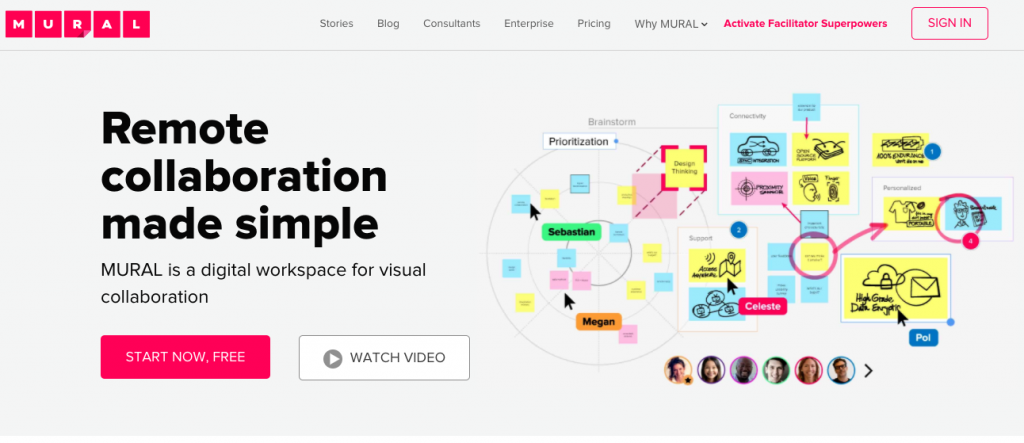
\includegraphics[width=1\linewidth]{img/mural.png}
  \caption{Mural homepage}
  \label{fig:mural}
\end{minipage}
\end{figure}

{\large
In spite of the existence of many web applications there is not a specifically designed tool for consultancy that could solve the problem of recording the meeting, analyzing what has been said, visualizing the data and displaying it to the user in an easy-to-understand way at the same time. One of the reasons why it has not been developed yet could be the fact that it is quite complicated to implement such a powerful tool.
}

\subsubsection{Summary}
{\large
Overall, consultancy has been developed with a start of Industrial Revolution and its progress peaked in \nth{21} century. The way of doing consultancy has not changed until the development of the internet and new technical tools. Whereas the Standard consultancy is still the prominent way to provide business expertise, e-consultancy is yet to be developed in a way of surpassing the old-fashioned way. On the other hand, meetings are already being held online what shows that it is only the matter of time when powerful tools will be developed and they will certainly get popular due to their efficiency and rapidity.\par

There is not really the wrong way of conducting a consultation. Whatever method that was ever used have always led to the same results, which simply could be described as achieving clients' targets and their goals.\par
}

\subsection{Speech Recognition}
\subsubsection{The History of Speech Recognition Technology}
\label{sec:dragon}
{\large
Speech recognition technology has become an integral part of our life, and with increasing popularity of home assistant systems it is more familiar than ever. Figure 3 shows that Amazon is the leading company in selling smart home products, while figure 4 shows estimated revenue for Amazon Echo speakers with Alexa over the years. Revenue is being almost doubled each year. These statistics show that the amount of people who rely on speech recognition devices increase every single year \parencite{amazonrules}, \parencite{alexastats}.\par
}

\begin{figure}[H]
\centering
\begin{minipage}{.5\textwidth}
  \centering
  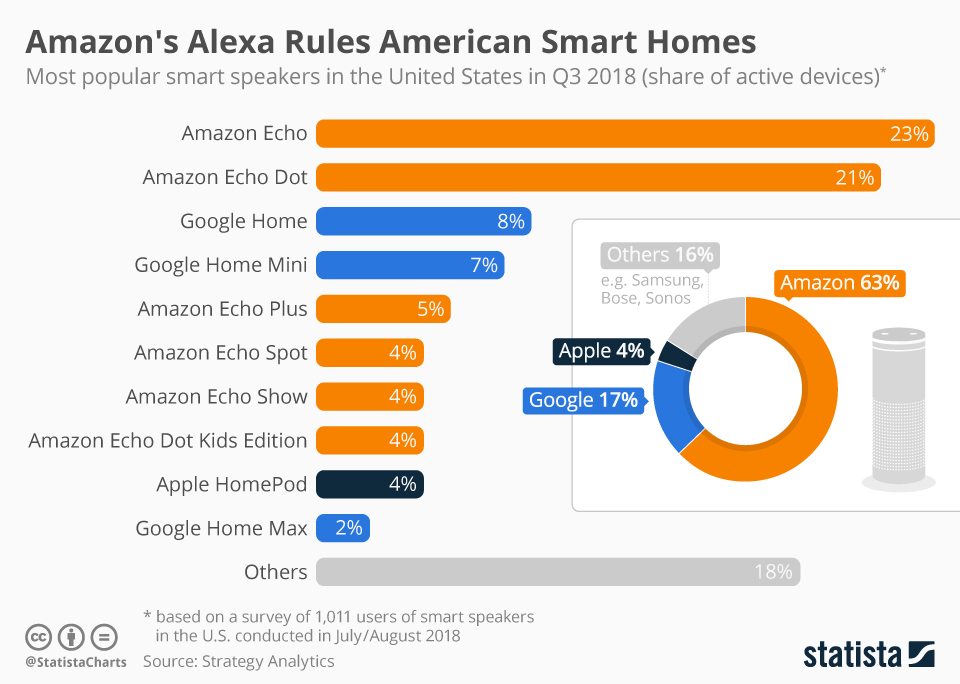
\includegraphics[width=0.97\linewidth]{img/amazonrules.jpg}
  \caption[Amazon's Alexa rules American smart homes]
    {\tabular[t]{@{}l@{}}Amazon's Alexa rules \\ American smart homes\endtabular}
  \label{fig:amazonrules}
\end{minipage}%
\begin{minipage}{.5\textwidth}
  \centering
  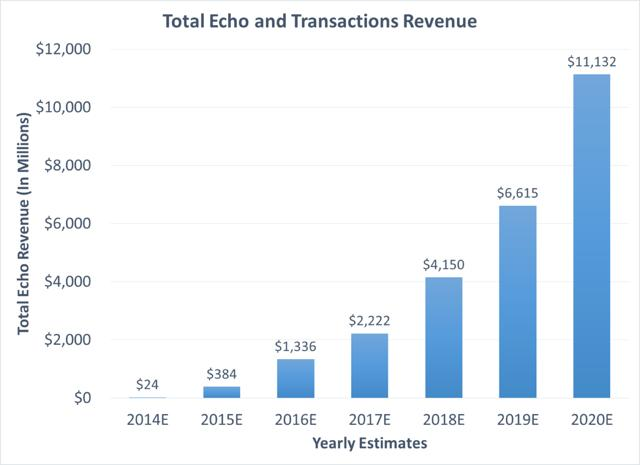
\includegraphics[width=0.97\linewidth]{img/alexastats.jpg}
  \caption[Total Echo and transactions estimated revenue by year]
  {\tabular[t]{@{}l@{}}Total Echo and transactions \\ estimated revenue by year\endtabular}
  \label{fig:alexastats}
\end{minipage}
\end{figure}

{\large
Despite a significant improvement in the voice recognition field in the recent years, there were many historical antecedents that have led to this point.\par
}

{\large
The first advance in speech recognition technology was aimed to interpret vowels and phonemes. Thanks to the great inventor Thomas Edison, dictations machines were created enabling to record speech quicker and easier.\par
}

\newpage
{\large
However, the first significant advance in speech recognition was created by Bell Labs in 1952. Labs invented what he called Audrey, a machine that could recognise the numbers from 0 to 9 with 90\% accuracy, but only using Lab's own voice. Whereas, the rate of accuracy would decrease when other person would speak to Audrey due to the differences of each individual’s tone, pace and voice. This was in fact, one of the challenges that speech recognition had to confront through its development.\par
}

{\large
In 1962 the company IBM created the Shoebox, a machine that was capable to identify 16 English words. During the 1970s the US Department of Defence and DARPA created Harpy, which could understand over 1000 words. In the 1980s the method called Hidden Markov Model (HMM) was established enabling to predict words with sounds. During this decade, the IBM machine Tangora was also created and could understand 20000 words. With the arrival of the 1990s speech recognition technology started to be accessible at work, thanks to Dragon Dictate, software that recognised 100 words per minute. This software is still in use nowadays.\par
}

{\large
During the first years of the 2000s, speech recognition technology did not evolve. It was not until 2008 that speech recognition became more popular with the creation of Google Voice Search. Three years after Google’s launch, Apple introduced Siri, a software that allows customers to manage different devices with the voice. The following years, companies such as Microsoft and Amazon created their own speech recognition devices.\par
}

{\large
Nowadays speech recognition technology is currently within the grasp of everyone making human being’s live easier and more comfortable. Figure \ref{fig:historyofspeechrecognition} shows the timeline of breakthroughs in speech recognition technology \parencite{historyofspeechrecognition}.\par
}

\begin{figure}[H]
  \centering
  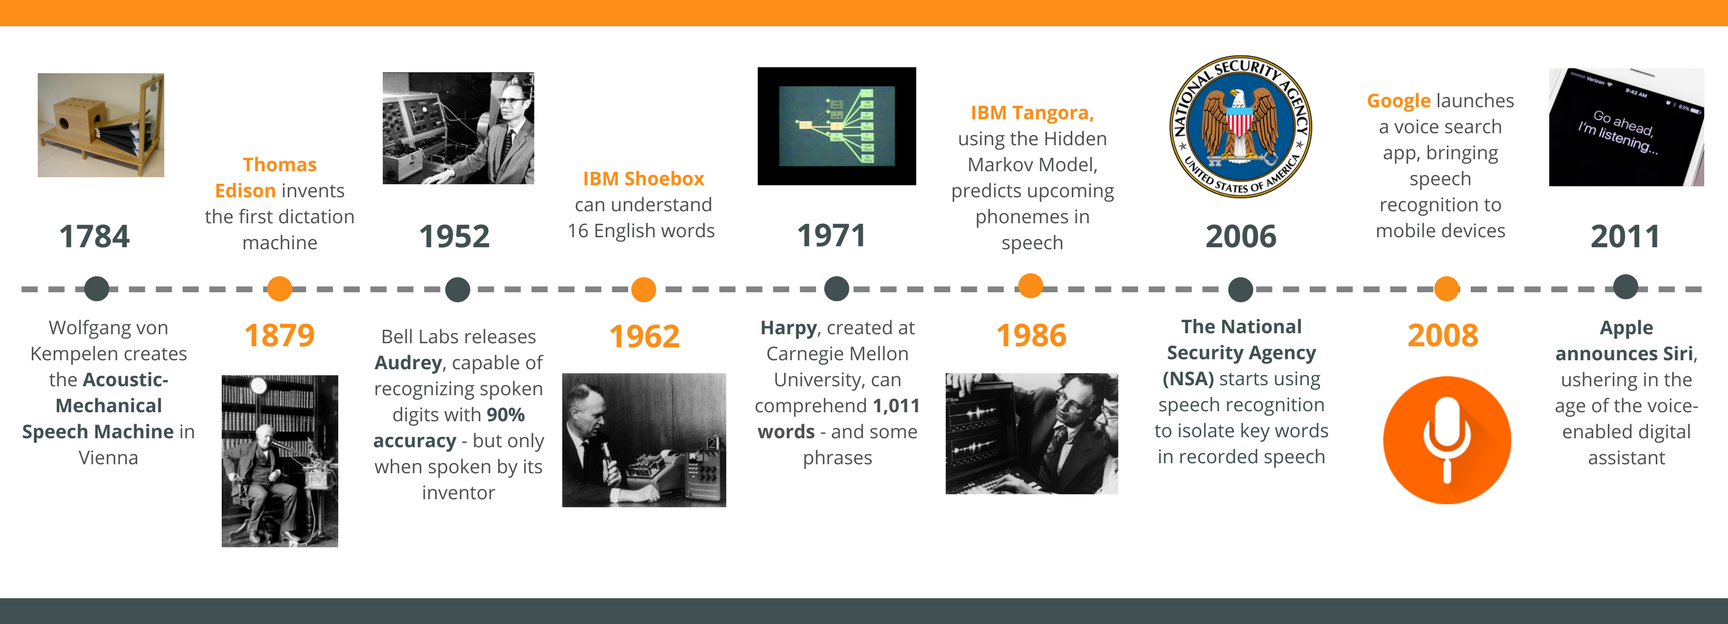
\includegraphics[scale=0.32]{img/speechrecognitiontimeline.png}
  \caption{Speech recognition technology timeline}
  \label{fig:historyofspeechrecognition}
\end{figure}


\subsubsection{The Models of Speech Recognition Systems}

\subsubsubsection{Dynamic Time Wrap}
\\
{\large
Dynamic Time Wrap is a template-based method, which means that speech is compared to another sequence of speech to find the optimal match and similarity between them. The sequences are "warped" non-linearly in the time dimension to determine a measure of their similarity independent of certain non-linear variations in the time dimension. Some of the advantages of DTW can be found in finding a match in speech sequences varying in speed as there are several ways in pronouncing the same word causing different time duration. This algorithm can analyse any data that can be turned into a linear sequence such as video, audio and graphics data. Dynamic Time Wrap is efficient for isolated word recognition and can also be used in connected word recognition \parencite{reviewofspeechrecognitiontechnique}.\par
}

\newpage

\subsubsubsection{Hidden Markov Model}
\\
{\large
Hidden Markov Model is one of the most used techniques in statistics and machine learning for modeling sequences speech in the field of natural language processing (NLP). It is a pattern recognition method, which involves pattern training and pattern comparison. This approach is modeled statistically by using
automatic, statistical learning procedure \parencite{reviewofspeechrecognitiontechnique}. It is assumed to be a Markov process – call it X – with unobserved ``hidden'' states. HMM assumes that there is another process y whose behavior "depends" on X. The goal is to learn about X by observing y. Probabilistic parameters of a hidden Markov model example:

\begin{figure}[H]
  \centering
  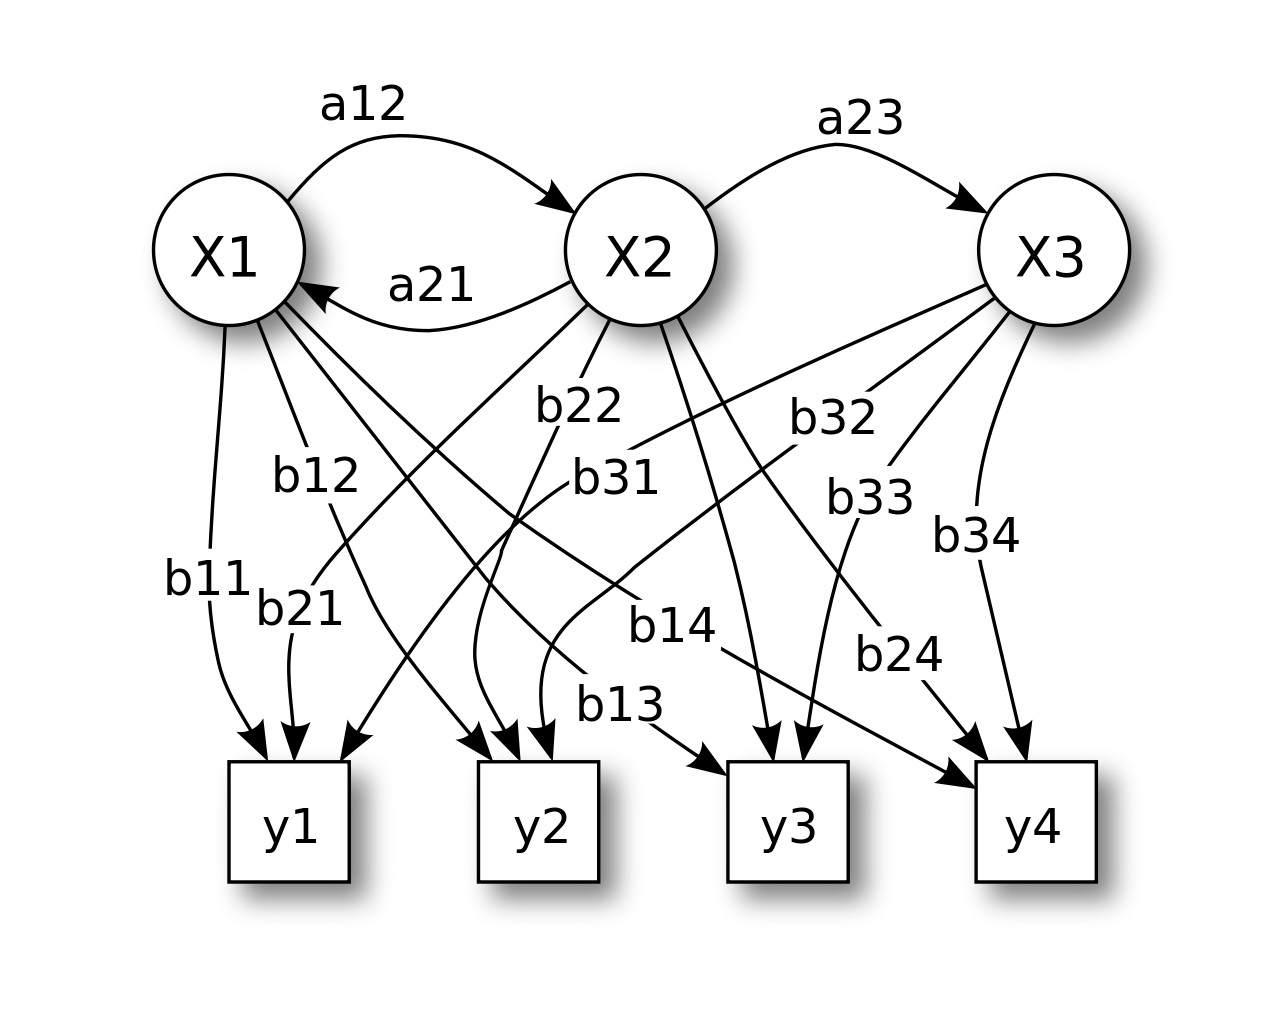
\includegraphics[scale=0.2]{img/hmm.png}
\end{figure}

where
\begin{conditions*}
    X & states\\
    y & possible observations\\
    a & state transition probabilities\\
    b & output probabilities\\
\end{conditions*}
One of the well known usage of HMM in speech recognition is Apple's Siri.
}

\subsubsection{Speech Recognition APIs \& Commercial Products}
\subsubsubsection{Google Cloud Speech-to-Text}
{\large
\\Google Cloud Speech-to-Text API accepts audio. It identifies speech in that audio and returns text representation of that speech. It all happens in real-time. It supports 71 languages and can detect up to 6 different speakers from the audio. Google mainly focuses on developing the machine learning service even further with constantly adding new features and making it more accessible. However, its features are mostly based on language instead of meaning and inference. Figure \ref{fig:googlestructure} shows the structure that Google uses for their multimedia transcription model, which is ideal for subtitling videos. It uses machine learning technology that is similar to video captioning on YouTube \parencite{googledocs}.\par
}

\begin{figure}[H]
  \centering
  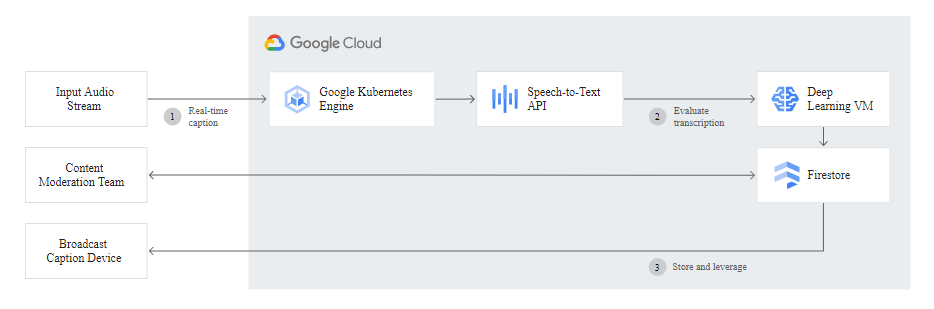
\includegraphics[scale=0.61]{img/googlestructure.png}
  \caption{Google Cloud: Transcribe multimedia content}
  \label{fig:googlestructure}
\end{figure}

\newpage

{\large
\begin{wrapfigure}{r}{0.65\textwidth}
  \vspace{-15pt}
  \begin{center}
    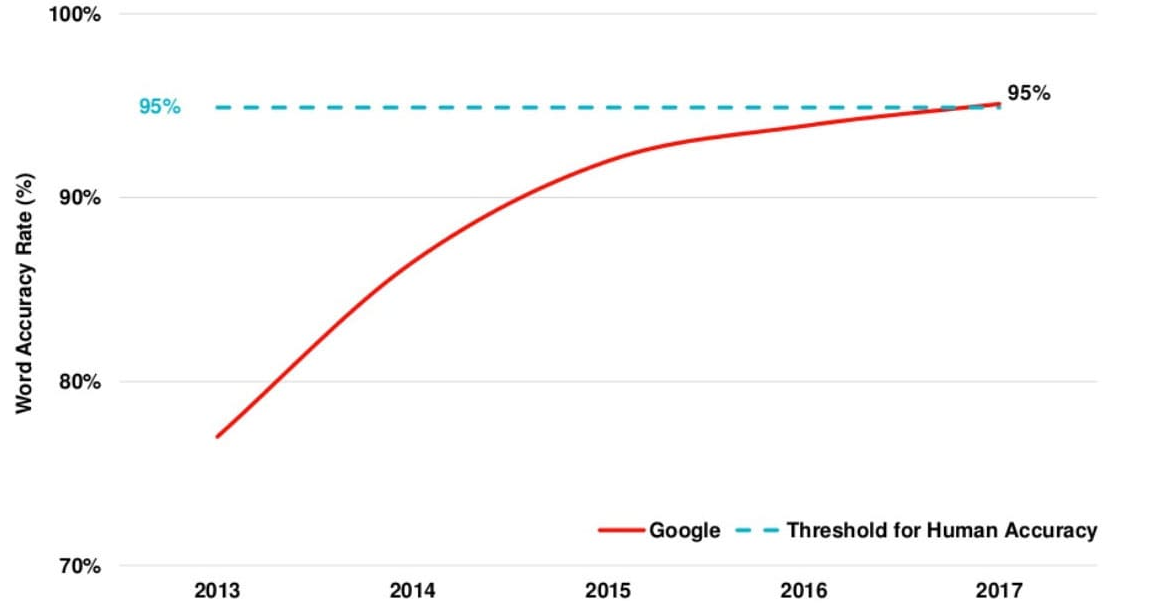
\includegraphics[width=0.65\textwidth]{img/googleaccuracy.png}
  \end{center}
  \vspace{-20pt}
  \caption[Google Machine Learning: Achieving Higher Word Accuracy, 2013-2017]
  {\tabular[t]{@{}l@{}}Google Machine Learning: Achieving higher word \\ accuracy, 2013-2017\endtabular}
  \label{fig:googleaccuracy}
  \vspace{-10pt}
\end{wrapfigure}
The graph in figure \ref{fig:googleaccuracy} plots Google’s word accuracy rate, which recently broke the 95\% threshold for human accuracy \parencite{googlespeechrecognition}. It could be the reason why many companies are deciding to use Google Cloud as their provider.\par
}

{\large
\begin{wrapfigure}{r}{0.45\textwidth}
  \vspace{-25pt}
  \begin{center}
    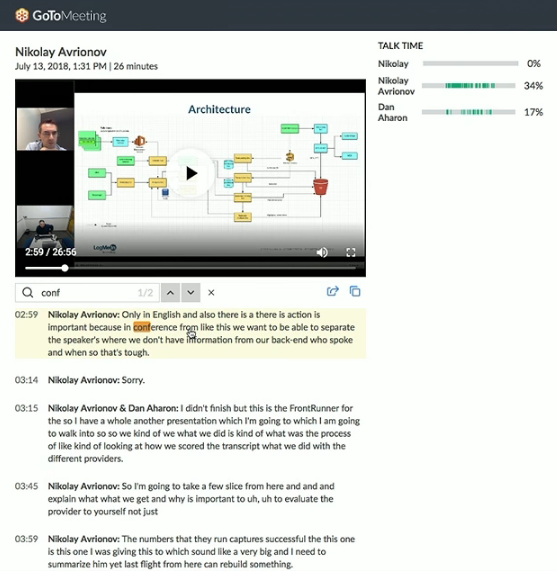
\includegraphics[width=0.45\textwidth]{img/gotomeeting.png}
  \end{center}
  \vspace{-20pt}
  \caption{GoToMeeting live transcript with search functionality and time management}
  \label{fig:gotomeeting}
  \vspace{-10pt}
\end{wrapfigure}
For instance GoToMeeting has selected Google as the provider of their speech transcription. Figure \ref{fig:gotomeeting} shows the functionality of the API and data post-processing \parencite{googleyt}. Other worth mentioning websites are speechnotes.co and dictation.io. Both of them have decided to use Google service to transcribe spoken words into text.\par
}
\vspace{40pt}
\subsubsubsection{Dragon Naturally Speaking}
\\
{\large
The previously mentioned in \hyperref[sec:dragon]{\textit{The History of Speech Recognition Technology}} Dragon Dictate became the software known today as Dragon Naturally Speaking. It is commonly used by users who might not be able to type for various reasons. In order to use the software, a user must first train the headset so that the program can know the way the user talks. During the training, the user has to read few paragraphs while the computer understands the way the user talks. Once training is complete, the user can begin talking and the program will translate the words into text. Nuance has also developed the medical version of the software, which allows doctors speaking directly into a patient’s electronic record. This software is mainly used by individuals rather than big companies, however the Nuance's speech recognition technology is recently focusing on in-car assistants too \parencite{dragoncar}.
\par
}

\subsubsubsection{Web Speech API}
\\
{\large
Web Speech API enables incorporating voice data into web applications \parencite{webspeechapidocs}. It can be used by JavaScript that gets the access to browser's audio stream through the API call. One of the most important factors of Web Speech API is that it is free and very accurate as it is using Google Cloud for the speech-to-text. The downside to it being gratis is that it is not known for how much longer it will stay free of charge, as well as the API is only supported by few browsers such as Google Chrome, Microsoft Edge and Samsung Internet mobile browser right now. Unfortunately, this service does not analyse the text and it does not differ speakers in conversation. These would need to be done in a post-processing.\par

\begin{wrapfigure}{r}{0.45\textwidth}
  \vspace{-20pt}
  \begin{center}
    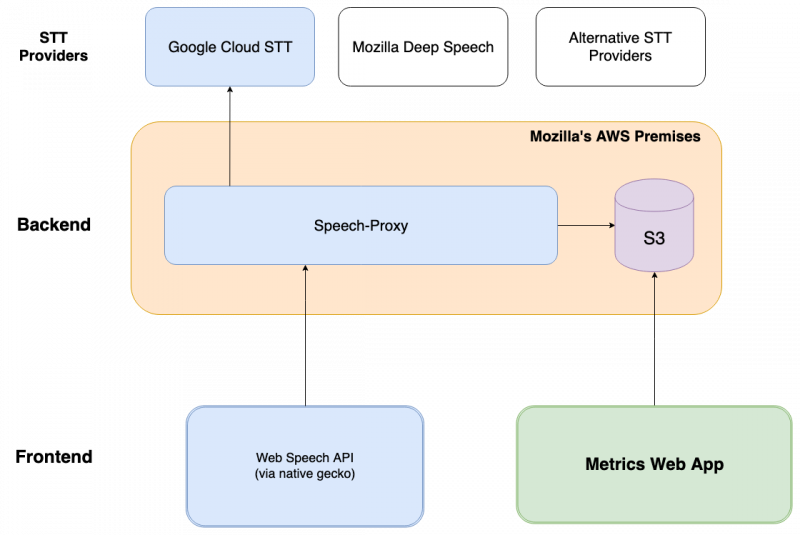
\includegraphics[width=0.45\textwidth]{img/webspeecharchitecture.png}
  \end{center}
  \vspace{-20pt}
  \caption{Web Speech API architecture}
  \label{fig:webspeecharchitecture}
  \vspace{-10pt}
\end{wrapfigure}
Figure \ref{fig:webspeecharchitecture} shows the current architecture of Web Speech API. Mozilla is currently developing their own service called Deep Speech, which is projected to be released in 2021 as a replacement for Google Cloud Speech-to-Text services. They are also considering using multiple speech recognition engines for different languages what could improve the word accuracy \parencite{webspeechapidocs2}.\par
}

\subsubsection{Speech Recognition Performance \& Benchmarks}
\subsubsubsection{Performance of Speech Recognition}
\\
{\large
There is not a single benchmark transcript used to test and evaluate a speech recognition system. Scripts are mainly picked by the tester knowing for what kind of services the system will be used. They can be audio from TV channels, YouTube, podcasts, meetings or specific recordings \parencite{wertest}. After generating transcripts they could be compared with the originally transcribed sources in order to benchmark the word accuracy by using test, widely known in the ASR field as Word Error Rate.\par

Another way to evaluate speech recognition performance is by timing the results of generated transcripts, however it is not used as much as WER, because it is more important to have more accurate system even if it could take more time.\par
}

\subsubsubsection{Word Error Rate}
\\
{\large
There are three types of incorrectly identified words that occur in speech recognition. Firstly, insertion means that there are incorrectly added words in the hypothesis transcript. Secondly, deletion stands for words that are undetected in the hypothesis transcript and finally substitution, so words that were substituted between reference and hypothesis. Figure \ref{fig:exampleofsdi} shows an example of these errors commonly known in speech recognition. \parencite{wererrors}

\begin{figure}[H]
  \centering
  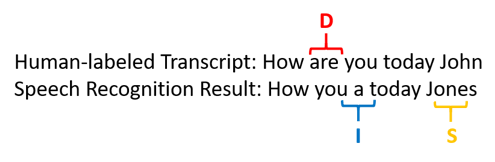
\includegraphics[scale=1.5]{img/wererrors.png}
  \caption{Example of substitution, deletion and insertion}
  \label{fig:exampleofsdi}
\end{figure}

Word error rate allows to evaluate the accuracy of a system \parencite{reviewofspeechrecognitiontechnique}. It is defined as
\[ WER = \frac{S + D + I}{N} \]
where
\begin{conditions*}
    S & number of substitution\\
    D & number of the deletions \\
    I & number of the insertions\\
    N & number of words in the reference\\
\end{conditions*}

WER of 5\%-10\% is considered to be good quality and is ready to use. Word error rate of 20\% is acceptable, however it might need an additional training, while a WER of 30\% or more shows poor quality and it requires customization and training of the system. Unfortunately, this method of evaluation also has some flaws. It ignores the importance of words, giving the same score for each error in a transcript. Another challenge comes with disregarding punctuation.

}
\subsubsection{Summary}
{\large
Nowadays speech recognition is widely used in many different fields including, but not limited to military, healthcare, transcription, robotics or even accessibility of many systems. There are many kinds of models and methods to recognise speech. DTW and HMM are examples of these recognition models. All of the presented APIs are commonly used to provide an excellent speech-to-text service, which mostly is very accurate. Each of these services already have the ability to convert speech to text and identify multiple users. What is more, they also allow user to tailor speech recognition models to adapt to users' speaking rules, expressions and unique vocabularies, as well as to accommodate background noises and different accents. On the other hand, they might differ when it comes to the number of languages they can process or the price for the provided service. Figure \ref{fig:table1} shows comparison of the data gathered in 2019 \parencite{table1}. It clearly states that Google has taken a lead in expanding the number of languages for the speech recognition technology.\par

\begin{figure}[H]
  \centering
  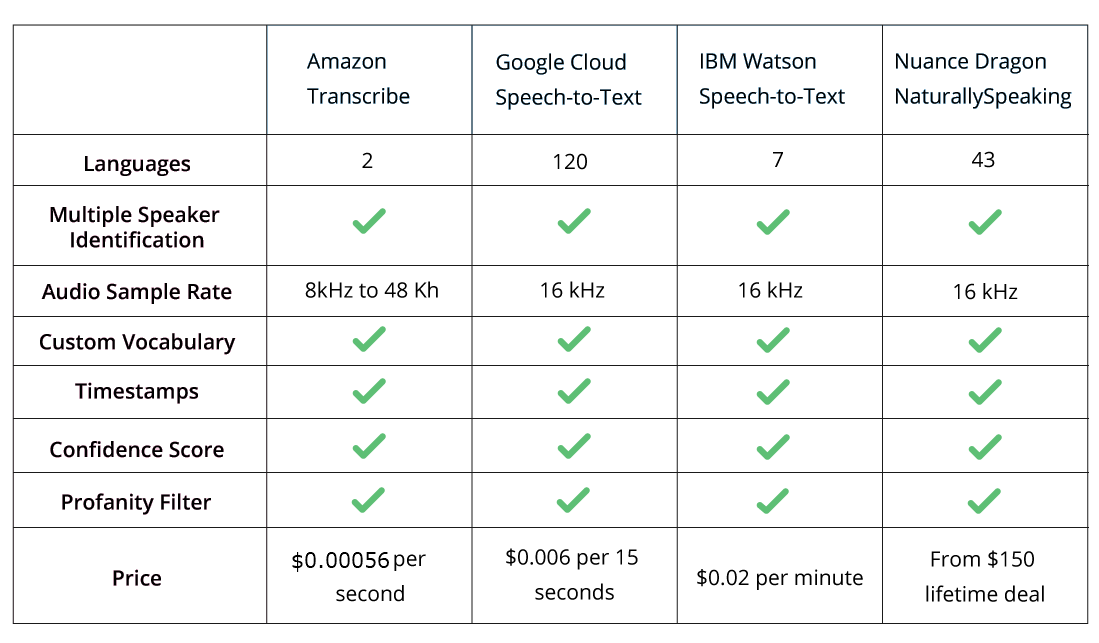
\includegraphics[scale=0.50]{img/table1.png}
  \caption{Comparison of Speech Recognition APIs}
  \label{fig:table1}
\end{figure}
}

\subsection{Existing Speech Recognition and Data Visualization Systems}
\subsubsection{TalkTraces: Real-Time Capture and Visualization of Verbal Content in Meetings}
{\large 
TalkTraces is a software developed to capture, analyse and represent the content discussed in meetings. The primary goal of the system is to help users to maintain an overview of current and prior discussion content. Users can proactively engage the display, filter discussion topics and review current conversations. Figure \ref{fig:talktraces} illustrates the way TalkTraces visualizes data \parencite{talktraces}.\par
}

\begin{figure}[H]
  \centering
  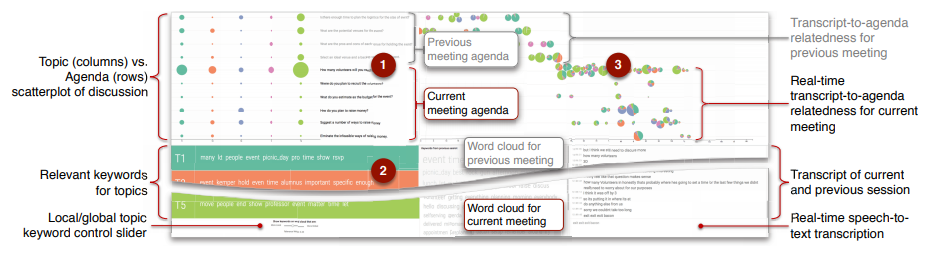
\includegraphics[scale=0.6]{img/talktraces.png}
  \caption{The final iteration of TalkTraces shows (1) agenda items from the previous and current meeting, (2) topics computed from the previous meeting transcript, and (3) transcript lines rendered as pie charts reflecting topic distribution, aligned with the most related agenda item.}
  \label{fig:talktraces}
\end{figure}

{\large 
Users, who tested the software found it difficult to keep track of topic-focused visualizations as the list of topics was updating all the time with different information. Participants suggested that reviewing topic-based visualization should be allowed only after the meeting or at a certain point of a conversation \parencite{talktraces}.\par
}

{\large 
The major limitation appears to be the predefinition of meetings' topics and agenda. Topics are picked up from the conversation, however they are compared with previously determined agenda items and compared to them. Unfortunately, talktraces are not analyzing the sentiment of the conversation in the meeting. The software is mostly focused on topic modelling instead.\par
}


\subsubsection{A Multimodal Real-Time Feedback Platform Based on Spoken Interactions for Remote Active Learning Support}
{\large 
The NAIRA application has been created to capture, store, analyse and visualize the spoken interactions of users in remote group activities. The software puts the most emphasis on improving the educational aspect of online meetings. Figure \ref{fig:naira} shows that the teacher can access an online dashboard with information such as effective time, silent time and influence graph that represents interactions between students \parencite{interactions}.\par
}

\begin{figure}[H]
  \centering
  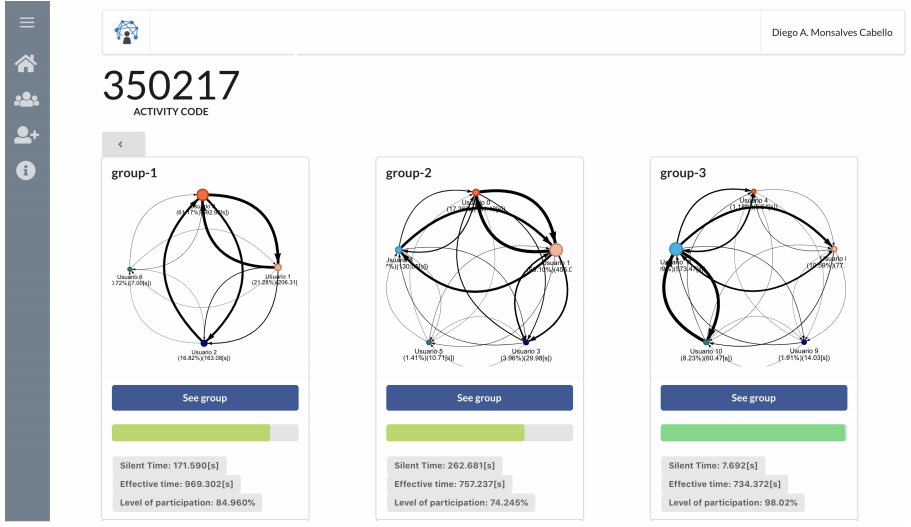
\includegraphics[scale=0.6]{img/naira.png}
  \caption{Teacher's view of dashboard in NAIRA application}
  \label{fig:naira}
\end{figure}

{\large 
Thanks to speaking time distribution, the teacher can recognise if in the group, there is any dominant student who concentrates a high percentage of the group's speaking time or if there is any passive student, who is mostly silent. This is when the teacher can engage appropriately with those students to increase productivity and collaboration in the group. Figure \ref{fig:naira2} shows the students' distribution of time: a) in the beginning of a group activity, b) after the intervention of the teacher, and c) in the end of the task \parencite{interactions}. This research has proven that speech recognition can be successfully used in a wide range of fields and how important it is to choose a right graph to display relevant data.\par
}

\begin{figure}[H]
  \centering
  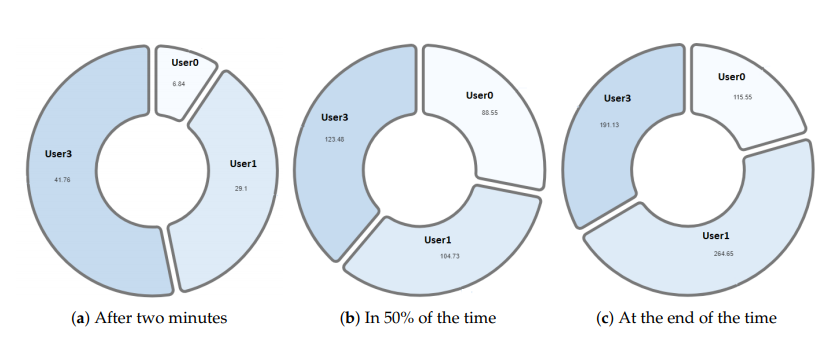
\includegraphics[scale=0.6]{img/naira2.png}
  \caption{Pie chart with the evolution of speech time distribution in a study group}
  \label{fig:naira2}
\end{figure}

\subsubsection{Sentiment Viz - Visualizing Twitter Sentiment}
{\large 
Sentiment Viz is a project, which studies ways to estimate and visualize sentiment of tweets posted on Twitter. After entering the keyword that has to be included in tweets, the software processes posted tweets from the last 24 hours and displays multiple graphs visualizing tweets sentiment, topics, occurring terms, timeline, map with locations from where they were sent and relation between them. Figures \ref{fig:sentimentviz} and \ref{fig:sentimentviz2} show how this project is using numerous visualization techniques to display graphs for ``speech recognition'' keyword. Every technique is designed to highlight different aspects of the tweets in a convenient way \parencite{twittersentiment}.\par
}

\begin{figure}[H]
  \centering
  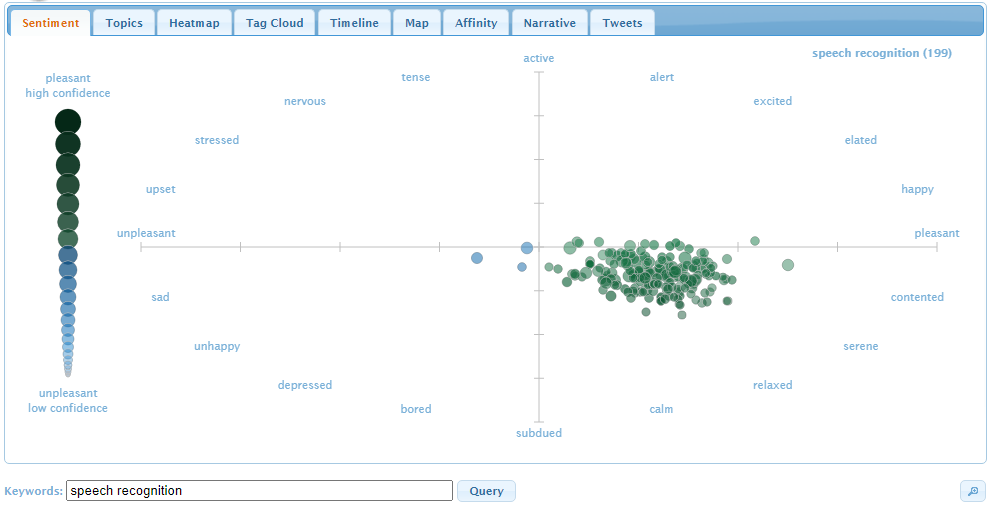
\includegraphics[scale=0.5]{img/sentimentviz.png}
  \caption{Sentiment visualization of tweets including ``speech recognition'' keyword}
  \label{fig:sentimentviz}
\end{figure}

\begin{figure}[H]
  \centering
  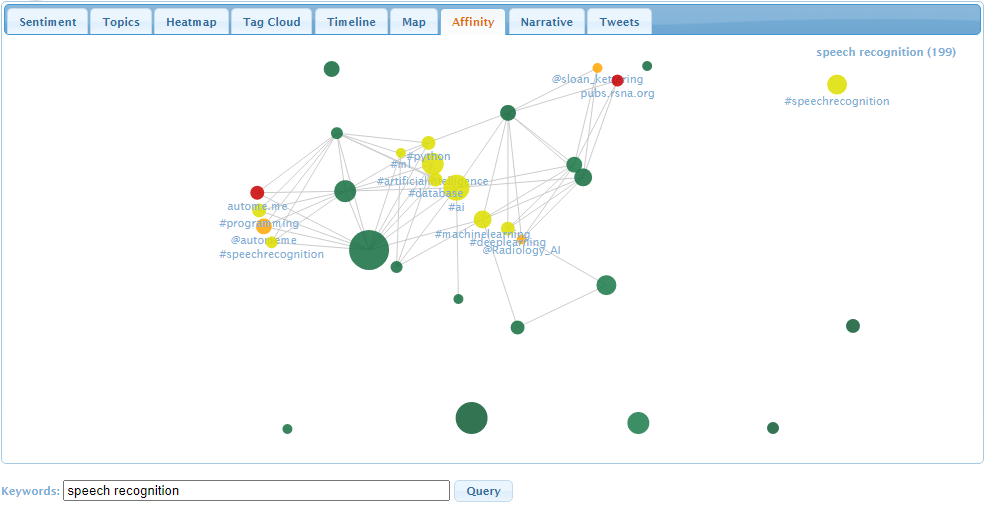
\includegraphics[scale=0.5]{img/sentimentviz2.png}
  \caption{Affinity visualization of tweets including ``speech recognition'' keyword}
  \label{fig:sentimentviz2}
\end{figure}

{\large 
The most interesting part in this study is that sentiment is not only shown as positive or negative, but as set of different emotional dimensions such as valence, arousal and dominance. Shankar found a way to use Affective Norms for English Words (ANEW) \parencite{bradley1999affective} to place words in different categories and display tweets with these words on a prepared graph visualizing the emotion conveyed by the particular tweet. Unfortunately, even this powerful tool has some scenarios, when it does not provide required results. For instance, a sentence ``We Been watching this sh*t for 2 hours n they been bashing Obama the whole time smh'' has been categorised as ``calm'', while it seems to be quite unpleasant, either stressed or tense. The result can be seen in figure \ref{fig:sentimentviz3} \parencite{shankar2011visualization}.\par
}

\begin{figure}[H]
  \centering
  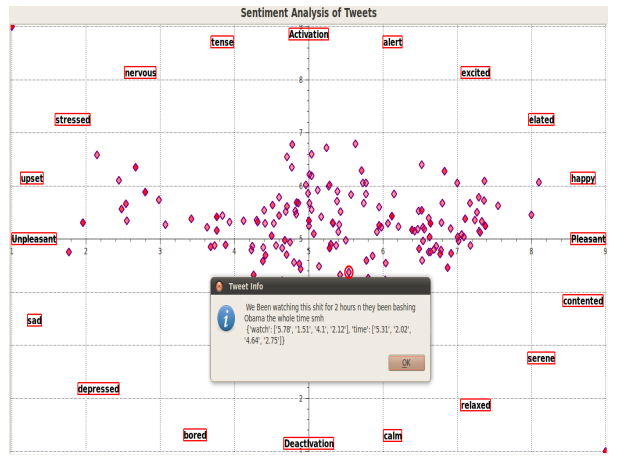
\includegraphics[scale=0.80]{img/sentimentviz3.png}
  \caption{Visualization of sentiments conveyed by tweets on ``Obama'' keyword}
  \label{fig:sentimentviz3}
\end{figure}

\subsubsection{Summary}
{\large
The research papers mentioned in this section are good instances of the recent advances in the field of combining automatic speech recognition with text analysis and visualization of spoken content. Each of the examples cover a big part of what eConsultant software will try to achieve, however they all have their limitations and different solutions to a similar problem.\par
}

\subsection{Text Analysis}
\subsubsection{Sentiment Analysis}
{\large
Sentiment analysis, also known as opinion mining is a way of using machine learning algorithms for natural language processing (NLP) and text analytics to identify parts of speech, sentiment, entities and other aspects of the text. It allows to understand textual data better and it determines whether it is positive, negative or neutral. Some of the services also detects mixed sentiment, which is a combination of a positive and negative sentence.\par

Sentiment analysis is mostly used for automated understanding of customer feedback in hospitality, retail and many more fields. Many companies use it to get an overview, because it is a quick and efficient way to know if customers' feedback is positive or negative, as well as finding out customers' attitude and emotions without having to read every single feedback. It can also be used in monitoring social media platforms, for instance Twitter to know if the certain topic is trending and what is being said about it.\par

Unfortunately, like in many other machine learning techniques there are some limitations. One of the problems that occurs would be identifying irony, jokes and sarcasm. People are very intuitive and would understand that sentences ``Well, what a surprise.'' and ``My flight’s been delayed. Brilliant!'' are sarcastic, while the sentiment analysis might determine these as positive.\par
}
\newpage
\subsubsection{Sentiment Analysis Techniques}
\subsubsubsection{Rule Based}
{\large
\\ This technique uses a dictionary of words also known as lexicons, which have labels with score of sentiment to determine the sentence. The rules are human-crafted what allows to identify subjectivity, polarity and the subject of an opinion. The technique is based on a frequency of positive-labeled and negative-labeled words in the text. If the number of positive words is higher than negative words, then sentiment is positive and vice versa. In case that the number of positive and negative words is even, then it means sentiment is neutral \parencite{monkey}.\par
}

\subsubsubsection{Machine Learning}
\label{sec:ml}
\begin{wrapfigure}{r}{0.6\textwidth}
  \vspace{-20pt}
  \begin{center}
    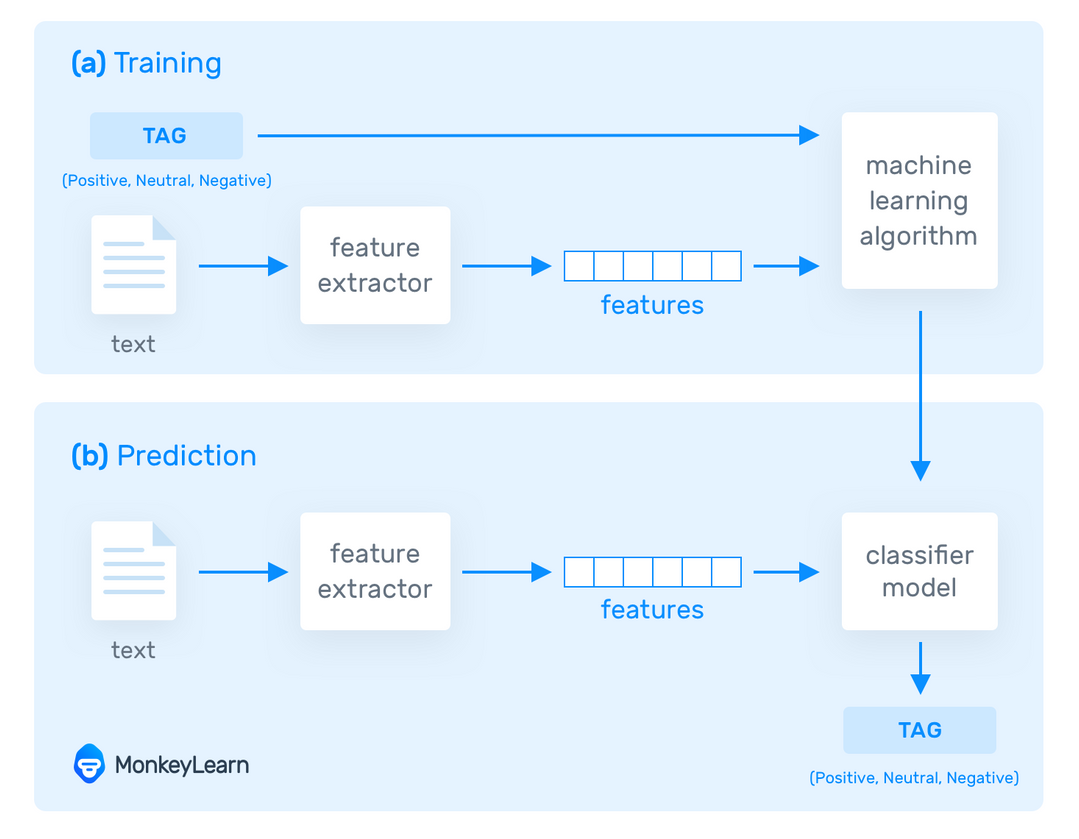
\includegraphics[width=0.6\textwidth]{img/monkey.png}
  \end{center}
  \vspace{-20pt}
  \caption{Example of machine learning classifier approach}
  \label{fig:monkey}
  \vspace{-20pt}
\end{wrapfigure}
{\large
This method is the contrary to rule based technique, it does not rely on manually chosen rules. As shown in figure \ref{fig:monkey}, the model is being trained to learn how to associate text to the corresponding sentiment based on the test samples used for training. Before the feature vectors are fed to the model to predict sentiment, they have to be created by transforming the text extraction into them. There has been a new feature extraction technique based on word vectors that allows words with similar meaning to have a similar representation, which improves the performance of classifiers. The classification part can involve a statistical model, however the most interesting approach lies in using deep learning instead. It uses a diverse set of algorithms that attempt to imitate the human brain by using artificial neural networks to process data \parencite{monkey}.\par
}

\subsubsubsection{Deep Learning}
{\large
\\As mentioned in the \hyperref[sec:ml]{\textit{Machine Learning}} subsection, deep learning is used to mimic the human brain. The model that has been dominating the most of the NLP tasks is long short-term memory (LSTM). It reads the text sequentially and keeps relevant information to the task at hand. While it is reading large amount of text, it is considered that LSTM is learning grammar rules. For instance, it learns the difference between ``bad'' and ``not bad''. The neural network will learn that it is important and will know which words could be negated \parencite{sentiment}.\par
}

\subsubsection{Text Analysis APIs}
{\large
There are plenty tools online that can do sentiment analysis of the text. The ones with the most accuracy in determining sentiment are AWS Comprehend, Google Cloud Natural Language and IBM Watson. Figure \ref{fig:sentimentapis} shows that the accuracy of sentiment detection in the most known services vary between 65\% and 68\%. It means they are all advancing at the same pace. What is also relevant and worth mentioning is that once these services are combined, the results of accuracy are increased by 7.4\% \parencite{sentimentapis}.\par
}

\begin{figure}[H]
  \centering
  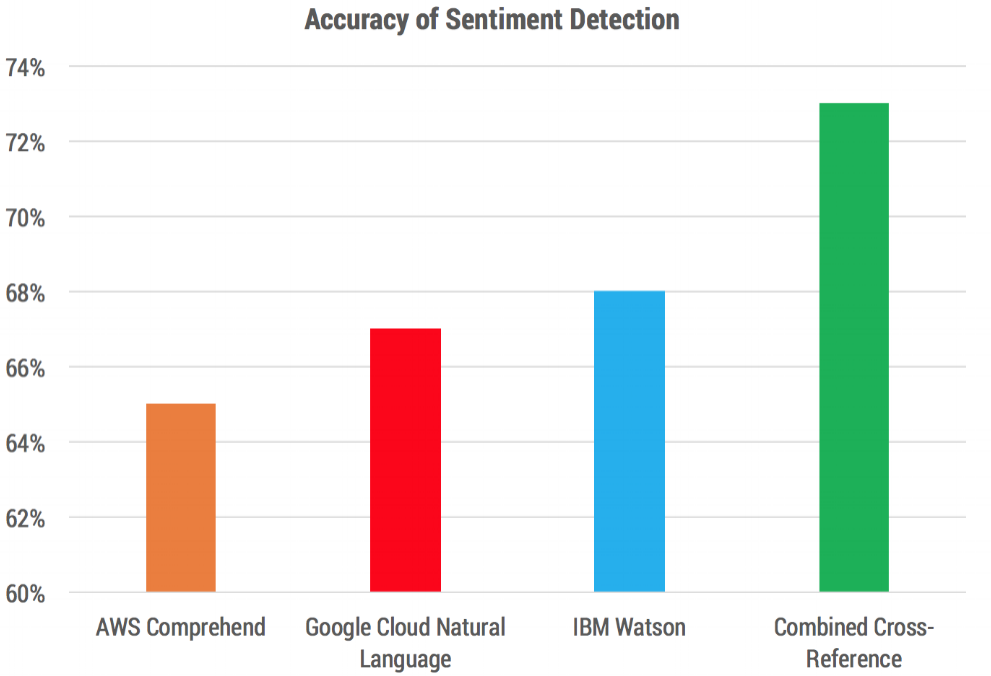
\includegraphics[scale=0.55]{img/sentiment.png}
  \caption{Accuracy comparison of sentiment analysis APIs}
  \label{fig:sentimentapis}
\end{figure}

\subsubsection{Summary}
{\large
Natural language processing has its role to play in the future of sentiment analysis. There is still a lot of work to be done, however improvements are being made every single day. It is possible that more companies will become aware of the features of sentiment analysis that can benefit them, and they might start using it to grow their business. Making this prediction leads to a summary that people will also realise that the phrase ``computer could think like a human'' becomes real.\par
}

\subsection{Data Visualization}
\subsubsection{The Art and Science of Data Visualization}

{\large
With the increasing popularity of computers and new advancements in visual design, graphic representation of data became more important. The techniques used in data visualization vary from simple bar charts and scatter plots to sophisticated multidimensional graphs and animations. Data visualization consists of two important parts, which can be recognised as the art and science. The first aspect of data visualization is the data itself, the information that is collected and processed. It is the scientific process, in which the information is gathered, identified and analysed using different statistical techniques and rules. The second aspect of it is the representation of that data, the translation of that information into a story making it understandable and interesting, what could be identified as artistic part.\par
}

{\large
Data science is a field that uses scientific methods and processes to prepare data for its visualization. It requires a specialist to conduct a research and extract the most appropriate insights from the data. It is a long process as using wrong data model could lead to a sloppy visualization.\par
}

{\large
There are four main considerations of the artistic aspect in drawing a chart or plotting a graph such as position, size, colour and shape. Combining these considerations in a right way can lead to a successful process of exploring the data. On the other hand, graph that looks uninteresting makes its data uninteresting too. Figures \ref{fig:goodchart} and \ref{fig:badchart} show the difference between good and bad example of data visualization. The map has a very intuitive, animated design and it is clear what the wind trends are without any need for numbers. The second chart is considered bad, because the author put too much effort in making it visually appealing and forgot about fundamental rules making the chart confusing. The size of the bubbles have no relationship with the values between them. Graph also creates an unintentional Venn diagram \parencite{goodchart}, \parencite{badchart}.\par
}

\begin{figure}[H]
\centering
\begin{minipage}{.5\textwidth}
  \centering
  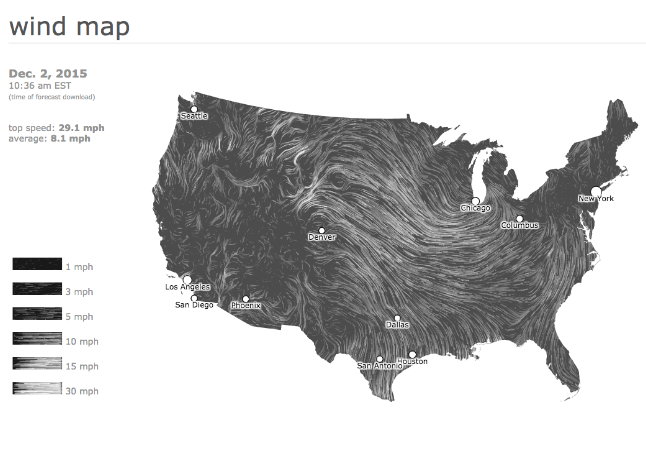
\includegraphics[width=0.97\linewidth]{img/goodvis.png}
  \caption[Good example of data visualization]
    {\tabular[t]{@{}l@{}}Good example \\ of data visualization\endtabular}
  \label{fig:goodchart}
\end{minipage}%
\begin{minipage}{.5\textwidth}
  \centering
  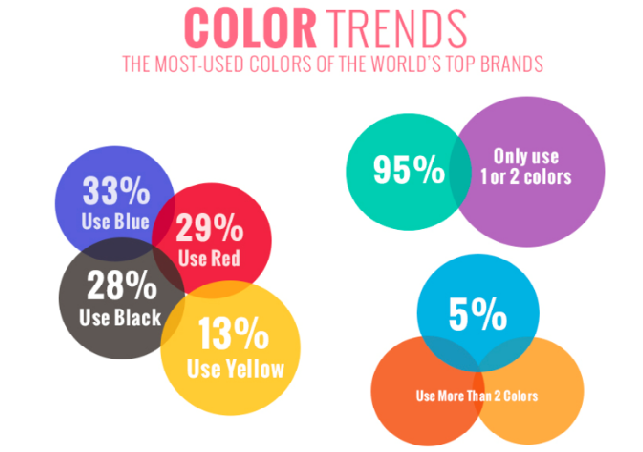
\includegraphics[width=0.97\linewidth]{img/badvis.png}
  \caption[Bad example of data visualization]
  {\tabular[t]{@{}l@{}}Bad example \\ of data visualization\endtabular}
  \label{fig:badchart}
\end{minipage}
\end{figure}

\subsubsection{Data Visualization in Consultancy}

{\large
Data Visualization is rarely used in consultancy, however it has few advantages why it might become a key role in the future. It can quickly point out something that deserves attention, make unexpected discoveries or build decisions based on facts displayed on various charts. The most promising charts could be the ones that highlight any sort of text analysis and time series displaying data evolution over time. Figures \ref{fig:powerbi} and \ref{fig:sankey} show instances of powerful diagrams that could be used and benefit consultancy field \parencite{sankey}, \parencite{powerbi}.\par
}

\begin{figure}[H]
\centering
\begin{minipage}{.5\textwidth}
  \centering
  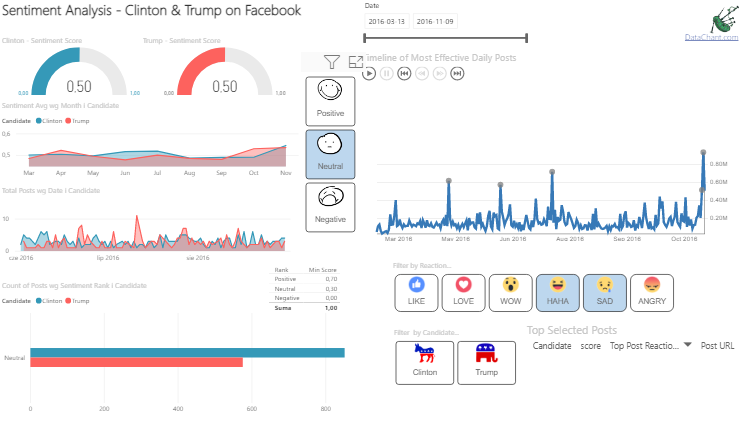
\includegraphics[width=0.97\linewidth]{img/consultancycharts.png}
  \caption[Sentiment analysis displayed on numerous graphs]
    {\tabular[t]{@{}l@{}}Dashboard with numerous \\ sentiment graphs \endtabular}
  \label{fig:powerbi}
\end{minipage}%
\begin{minipage}{.5\textwidth}
  \centering
  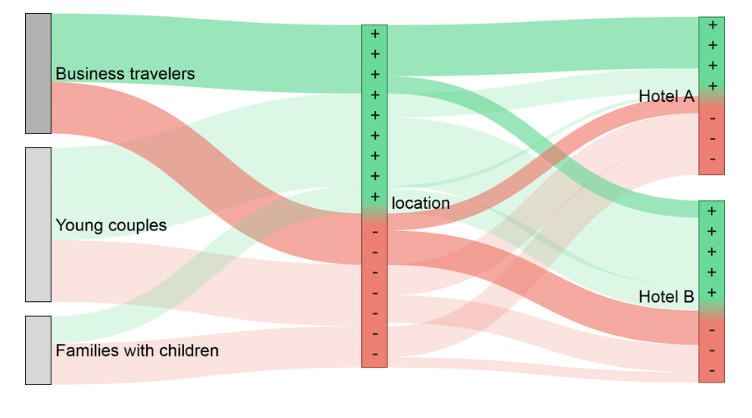
\includegraphics[width=0.97\linewidth]{img/sankeychart.png}
  \caption[Sentiment displayed on sankey diagram]
  {\tabular[t]{@{}l@{}}Sentiment displayed on sankey diagram \\ showing positive and negative reviews\endtabular}
  \label{fig:sankey}
\end{minipage}
\end{figure}

\subsubsection{Summary}
{\large
Data visualization is a place where science meets art, however data specialists still wonder whether it is a more artistic effort or a scientific one. In spite of the fact that experts agree that a compelling visual requires both, it is not commonly agreed if science comes before design. It depends on who is creating the visualization, and who the audience is. It does not change the fact that data visualization is very important nowadays and having a good understanding of it can be crucial for businesses to make the right decision.\par
}

\newpage
\subsection{Conclusion}
{\large 
In conclusion, this review has described technologies and ample of studies related to speech recognition, sentiment analysis and data visualization. There is not a single system that combines these three fields, which could facilitate an online meeting and be specifically used in the field of consultancy. For the development of this project, Web Speech API could provide speech to text transcription as it is using Google Cloud API that has the highest word accuracy. There is also plenty of approaches in doing text analysis, however the most used method is machine learning, because it is the most accurate and it is used by service providers such as Amazon Comprehend, which provides more than enough features to be used in this project for sentiment analysis, key phrases and entities extraction. Amazon Web Services also provides DynamoDB, which could be a reliable database for storing meetings' information and conversation. Data visualization is a very wide field and it uses many different charts and graphs for different type of data. Carefully chosen visual representation of data could help in developing the admin dashboard used for seeing an overview of the meeting. Technological advances in all these areas that have been proved in the previous chapter make it feasible to develop a desired web application.\par
}

\newpage

\section{Design}

\subsection{System Description}
{\large 
The objective of this project was to create a speech to text, sentiment analysis data visualization application that can be used during consultancy meetings. It can make consultant job more effective with this automation. Something that would be done by one or few consultants, now can be done by this software. Making sure that meetings' participants stay on the meetings' agenda is only one of many examples of what the system is capable of. As the background research has proven, such tool had not been implemented yet and all the stakeholders could benefit from the existence of the software itself. After recording the spoken content of the meeting, the speech is being sent to the transcription cloud service that gives back raw text which is interpreted and analysed with Amazon Web Service. The findings from the text are available on the administrator dashboard. The overview of the data is visualized and displayed on various charts.\par
}

\subsection{Stakeholders}
{\large 
In this project, the internal stakeholders include module leader, my supervisor Dr. David Gamez and Sarah Braid, who is financially supporting the development. After making an official release of the commercial product, it could be used by many users. It means there would also be external stakeholders such as customers and participants of the meetings. Involvement of investors would also qualify as having them as internal stakeholders.\par
}

\newpage
\subsection{Requirements Specifications \& Technology Choices}
{\large 
\begin{enumerate}
    \item System running in the cloud to facilitate small and large meetings
        \begin{itemize}
        \item Achieved by choosing Amazon Web Services as cloud provider
        \end{itemize}
    \item Individually recording speech of all people in a meeting
        \begin{itemize}
        \item Users must have their own microphones if the meeting is held online
        \item Converting speech to text with Web Speech API
        \item Using Punctuator API to punctuate raw text received from Web Speech API
        \end{itemize}
    \item Storing text in the database
        \begin{itemize}
        \item Accomplished with Amazon DynamoDB
        \end{itemize}
    \item Analyse the conversation
        \begin{itemize}
        \item Using Amazon Comprehend for sentiment analysis and extraction of key phrases to find the topics of the meeting
        \end{itemize}
    \item Connecting meeting topics with other company documents
        \begin{itemize}
        \item Another useful usage of Amazon Comprehend for extracting entities
        \end{itemize}
    \item Implementation of clean UI to avoid creating new user experience problems
        \begin{itemize}
        \item Accomplished with Architect-UI template
        \end{itemize}
    \item Having administrator accounts to access the dashboard
        \begin{itemize}
        \item Achieved with Amazon Cognito
        \end{itemize}
    \item Creating dashboard with data visualization of all the information
        \begin{itemize}
        \item Build with JavaScript charting libraries such as ZingChart.js, amCharts.js and Plotly.js
        \end{itemize}
\end{enumerate}
}

\subsection{Use Case}

{\large 
Figure \ref{fig:Use Case} depicts the use case diagram example, in which the user is joining the meeting. It would not be possible without the administrator, who can access dashboard in order to create a meeting. All other actions can be taken independently. Once user attends the meeting, his speech is being recorded and administrator is able to view the charts related to the particular meeting. Administrator is also able to upload documents to see if there is a connection between them and the meeting. After the completion of the gathering, administrator can conclude it by closing the meeting.\par
}
\vspace{10pt}
\begin{figure}[H]
  \centering
  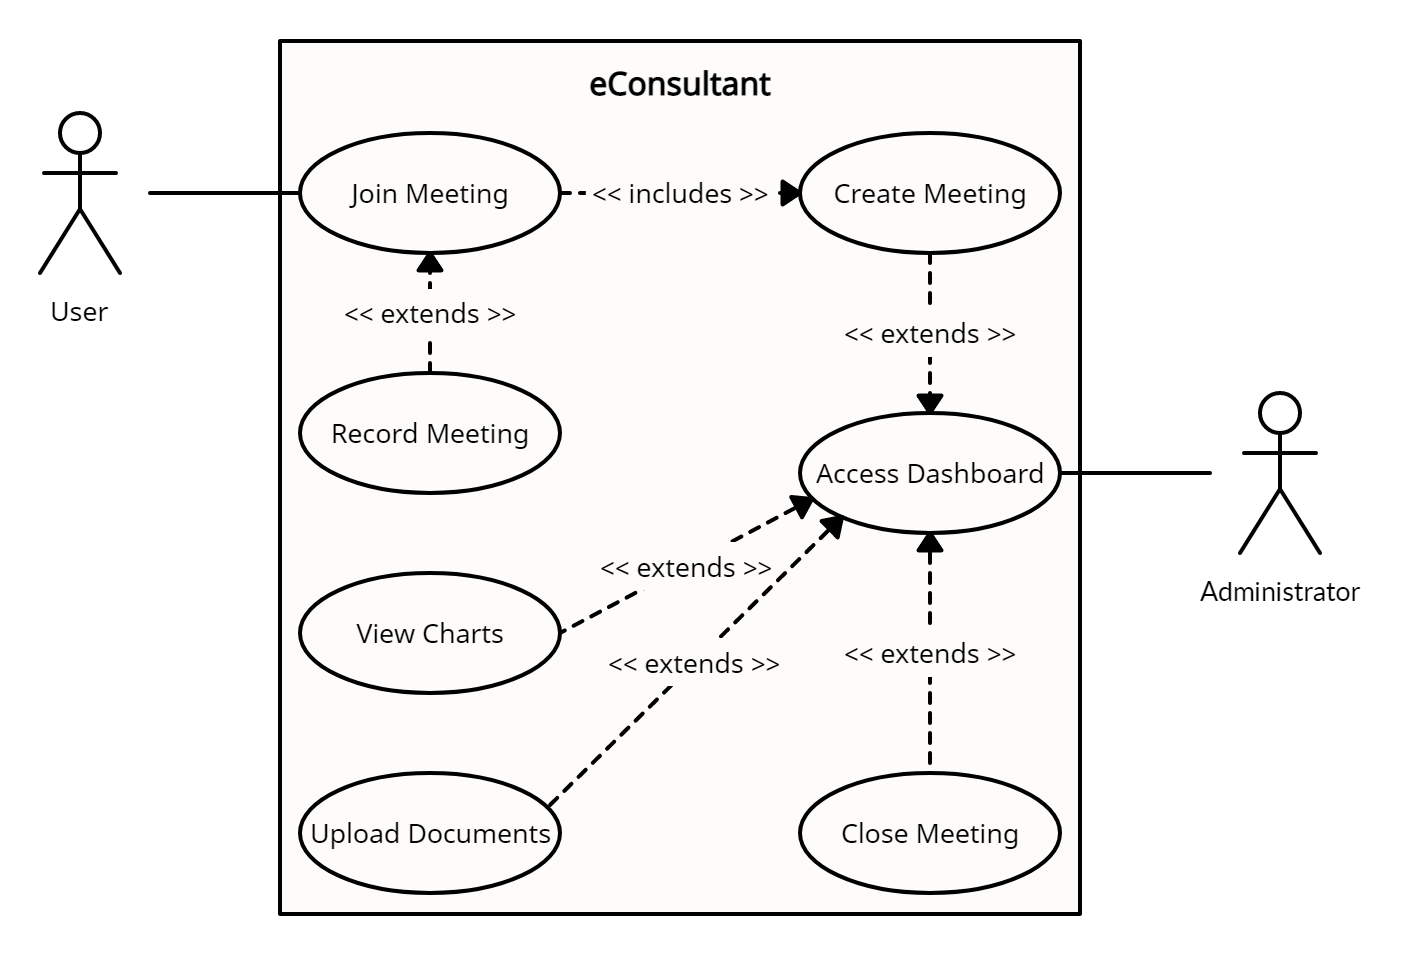
\includegraphics[scale=0.3]{img/usecase.png}
  \caption{Use Case}
  \label{fig:Use Case}
\end{figure}

\subsection{System Architecture}
{\large
EConsultant is build on Node.js server by using Express.js. It is hosted on the Amazon EC2 instance, so that the software is available from any location at any time. Amazon Cognito allows administrator to access the dashboard as well as ``saving resources'' page. The server allows flawless communication between client, database and other third party services. User's speech is being sent to Google Cloud Speech Recognition Standard API via Web Speech API. Received text is later send to Punctuator API to apply punctuation to raw text. Punctuated text is analysed with Amazon Comprehend. Finally, the analysed data is being stored in Amazon DynamoDB so it can be retrieved and sent back to the user.\par
}
\begin{figure}[H]
  \centering
  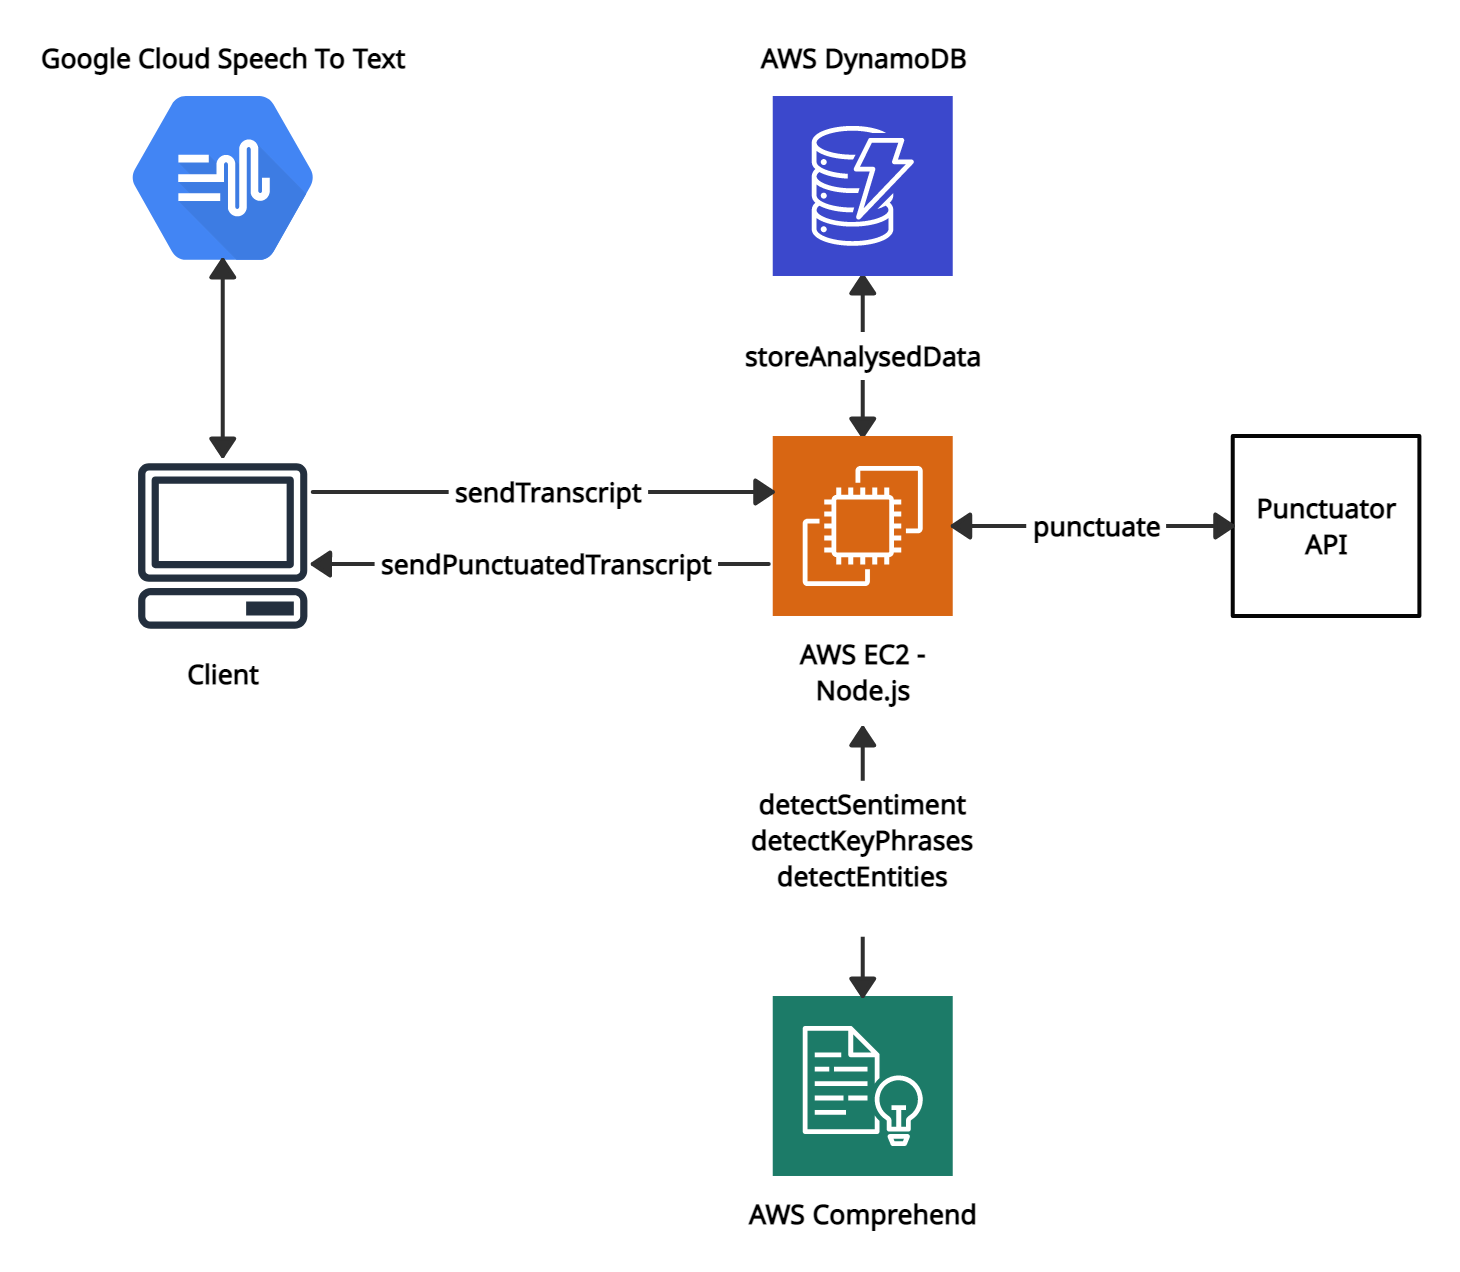
\includegraphics[scale=0.26]{img/architecture.png}
  \caption{System Architecture}
  \label{fig:System Architecture}
\end{figure}

\subsection{Database Design}

{\large
Amazon DynamoDB is a non-relational database, however it is still a good practice to define an ER diagram, it is shown in figure \ref{fig:Database Design}. It establishes the entities and their relationship to one another in a database-agnostic way. Redundancies have been eliminated by conducting some steps of the normalization process. There are three tables, which include ``Meetings'', ``Messages'' and ``Documents''. Primary keys are displayed in bold. Both, ``meetingName'' from ``Messages'' table and ``meetingName'' from ``Documents'' table are foreign keys of ``name'' from ``Meetings'' table. They are one-to-many relations.\par
}
\vspace{10pt}
\begin{figure}[H]
  \centering
  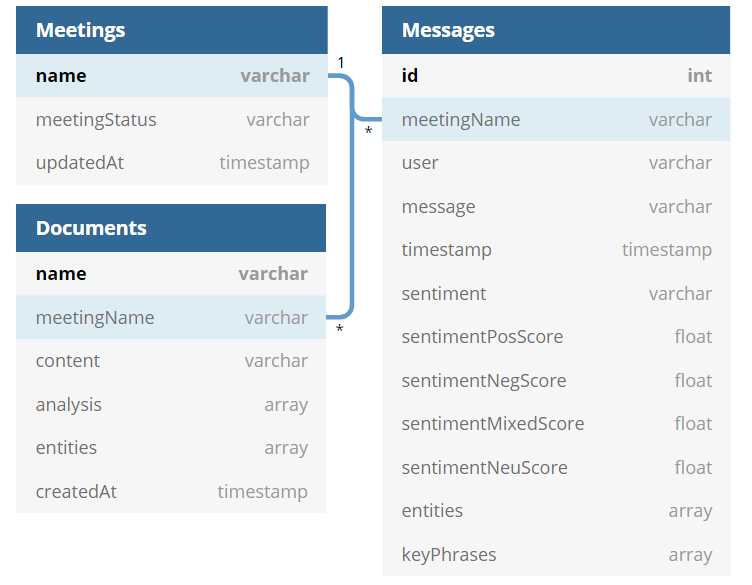
\includegraphics[scale=0.7]{img/dbdesign.png}
  \caption{Database Design}
  \label{fig:Database Design}
\end{figure}

\subsection{Wireframes}

\begin{figure}[H]
\centering
\begin{minipage}{.5\textwidth}
  \centering
  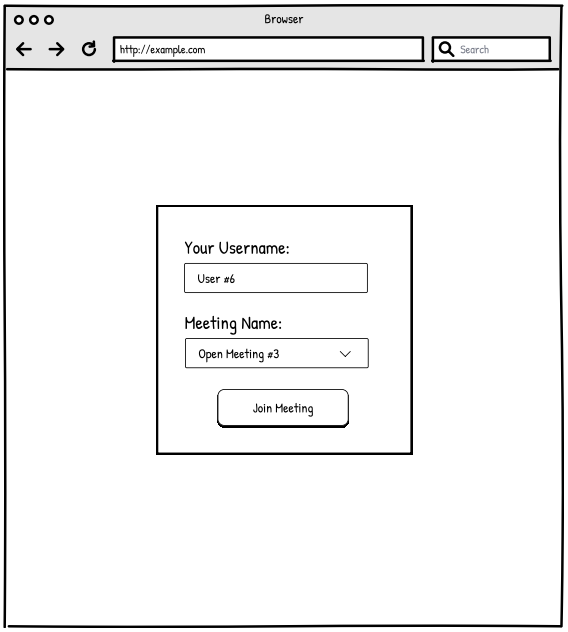
\includegraphics[width=0.97\linewidth]{img/join.png}
  \caption{Join meeting page}
  \label{fig:join}
\end{minipage}%
\begin{minipage}{.5\textwidth}
  \centering
  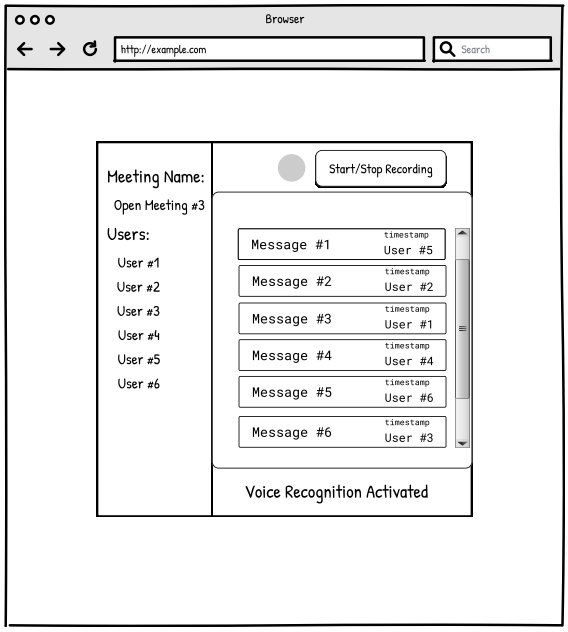
\includegraphics[width=0.97\linewidth]{img/meeting.png}
  \caption{Meeting page}
  \label{fig:meeting}
\end{minipage}
\end{figure}

\begin{figure}[H]
  \centering
  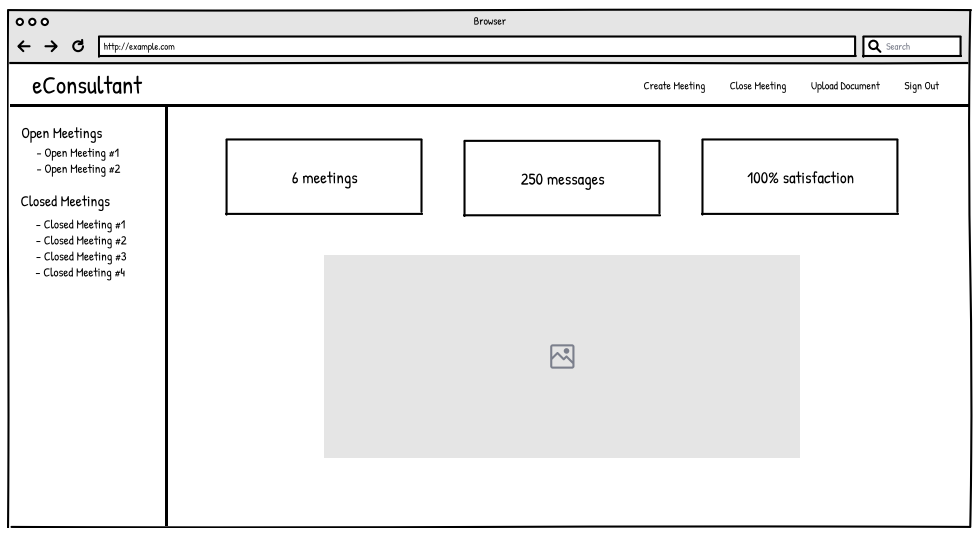
\includegraphics[scale=0.57]{img/home.png}
  \caption{Dashboard wireframe}
  \label{fig:Home Page}
\end{figure}

\begin{figure}[H]
  \centering
  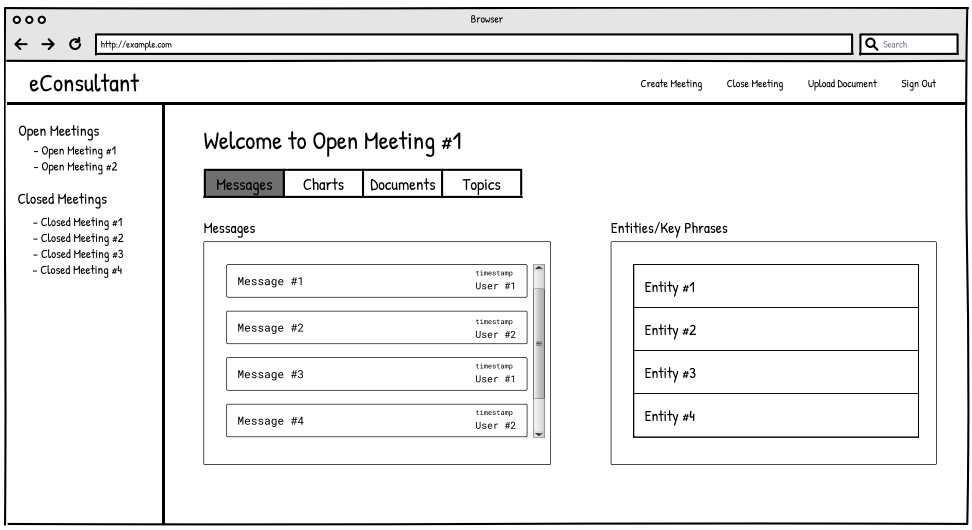
\includegraphics[scale=0.57]{img/messages.png}
  \caption{Messages tab wireframe}
  \label{fig:Messages tab}
\end{figure}

\begin{figure}[H]
  \centering
  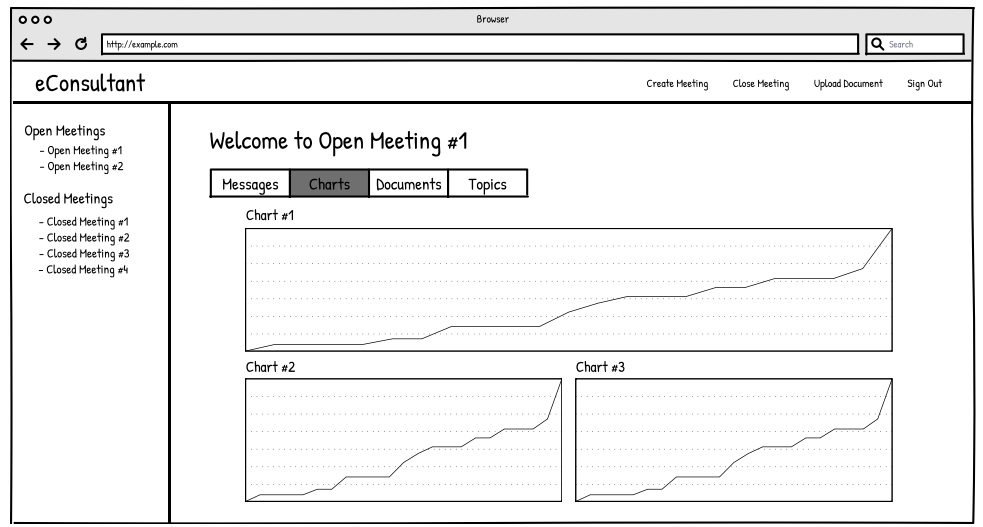
\includegraphics[scale=0.57]{img/charts.png}
  \caption{Charts tab wireframe}
  \label{fig:Charts tab}
\end{figure}

\begin{figure}[H]
  \centering
  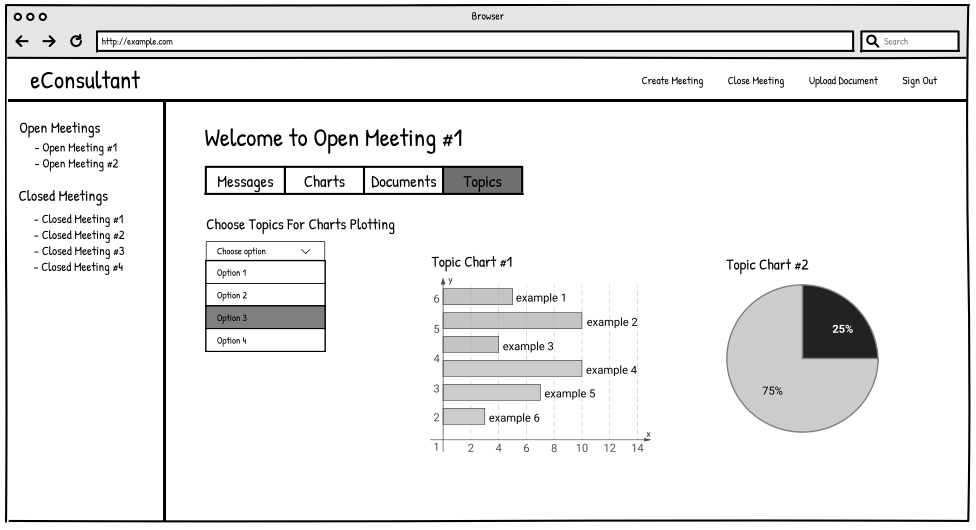
\includegraphics[scale=0.57]{img/topics.png}
  \caption{Topics tab wireframe}
  \label{fig:Topics tab}
\end{figure}

\newpage

\section{Implementation}
{\large 
EConsultant development has been completed and all requirements have been considered and met. This web application is an useful tool that a consultant can use to facilitate their meetings. There was not any change in respect to the design chapter, however additional single page hosted on Amazon S3 bucket has been added to save the resources from Amazon Web Services account. It is also using Amazon Cognito for authentication for administrator. This chapter will explain the process of creating the website and implementing the functionality of the product.\par
}

\subsection{Meeting's Chat}
{\large 
Users can join the meeting by entering their names and choosing the meeting from the drop-down menu. After selecting the information users will be redirected to the meeting's chat. Chat shows all the messages spoken in the meeting and the information about the new people joining it. The side component of the chat displays the name of the actual meeting and the user names actively attending the meeting. The button allows turning on listening to the user's microphone as it is set to be off by default when joining the meeting. These two pages have been implemented with Socket.IO and Web Speech API. Figures \ref{fig:joinMeetingPage} and \ref{fig:meetingPage} show discussed features.\par
}

\begin{figure}[H]
  \centering
  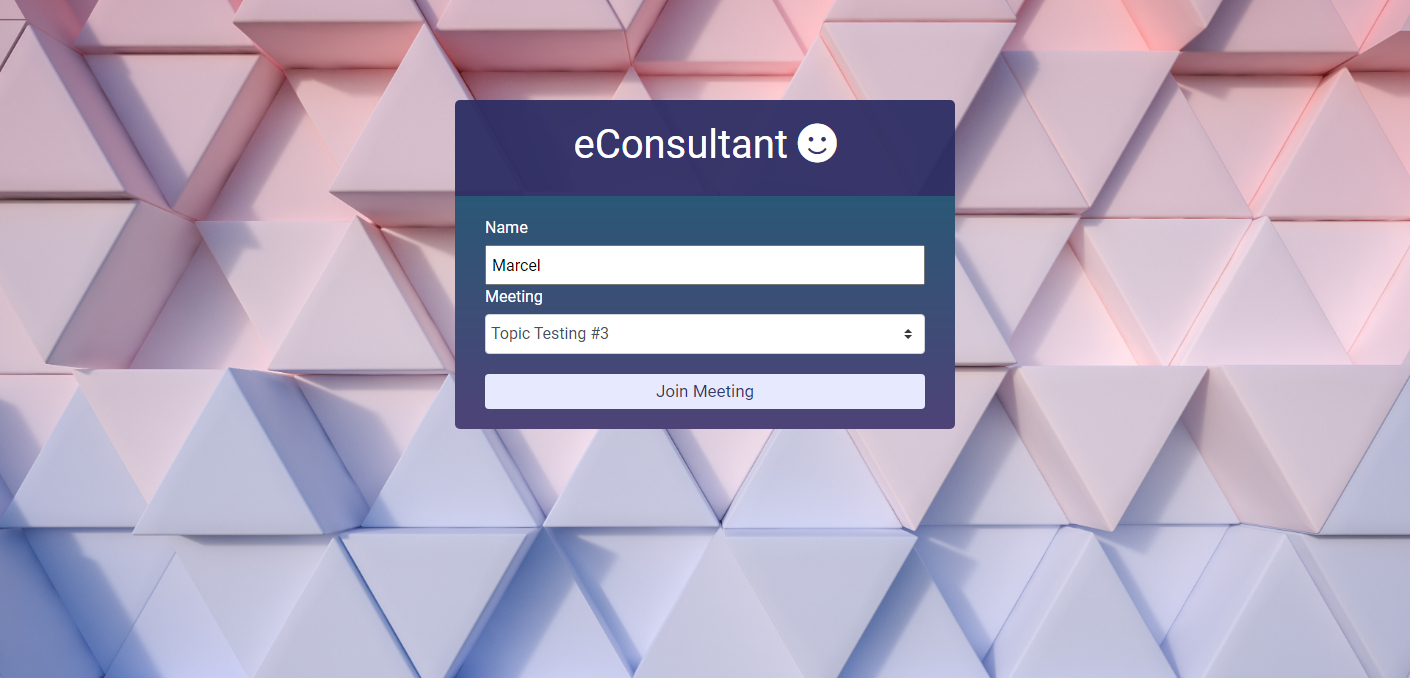
\includegraphics[scale=0.29]{implementation/joinMeeting.jpg}
  \caption{Join meeting page}
  \label{fig:joinMeetingPage}
\end{figure}

\begin{figure}[H]
  \centering
  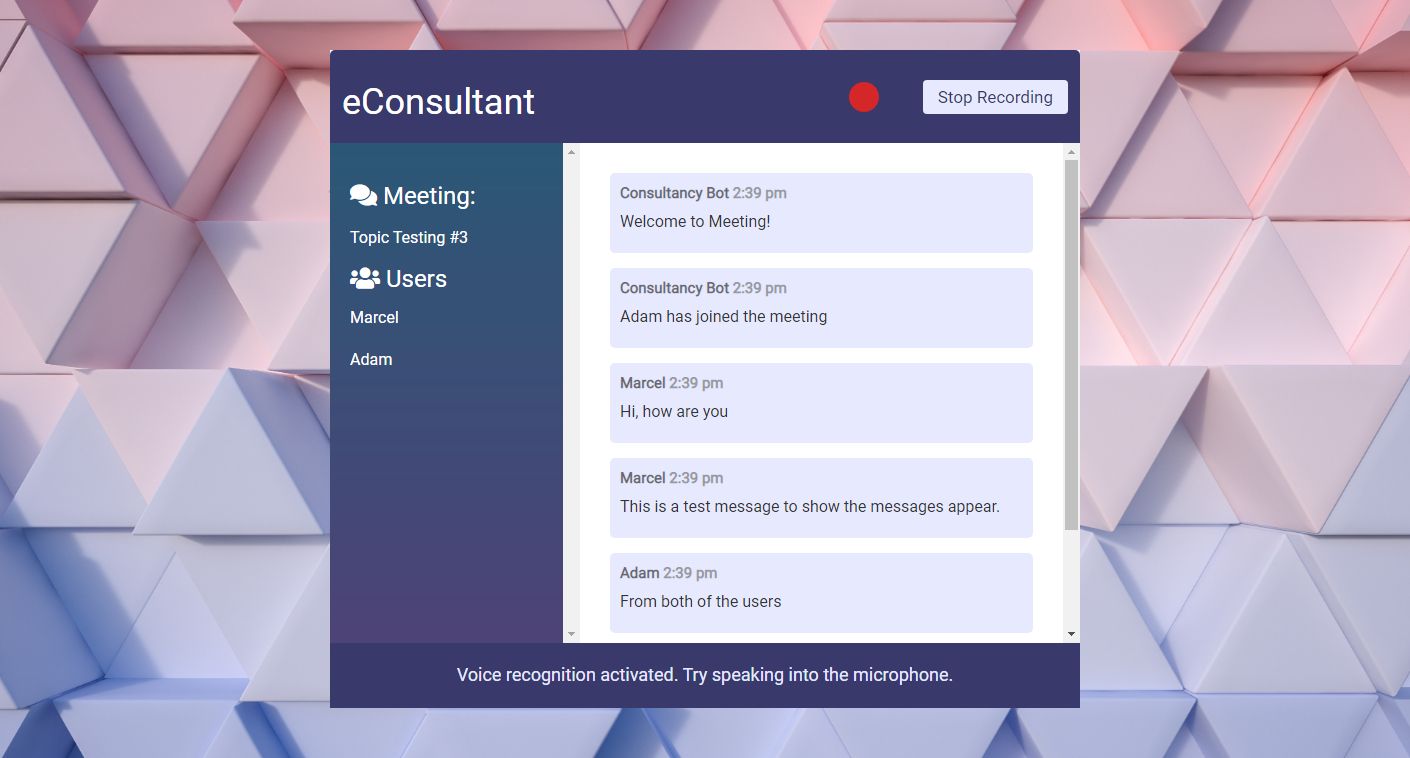
\includegraphics[scale=0.29]{implementation/meeting.jpg}
  \caption{Meeting page}
  \label{fig:meetingPage}
\end{figure}

\subsection{Administration Dashboard}
{\large 
Administrators can access the dashboard which allows to perform various tasks, however the first thing before being able to access the page is filling up login details. Login has been implemented with Amazon Cognito service, it is shown in figure \ref{fig:login}. If credentials are incorrect the validation message is displayed to the user in red colour. \par
}

\vspace{15pt}

\begin{figure}[H]
  \centering
  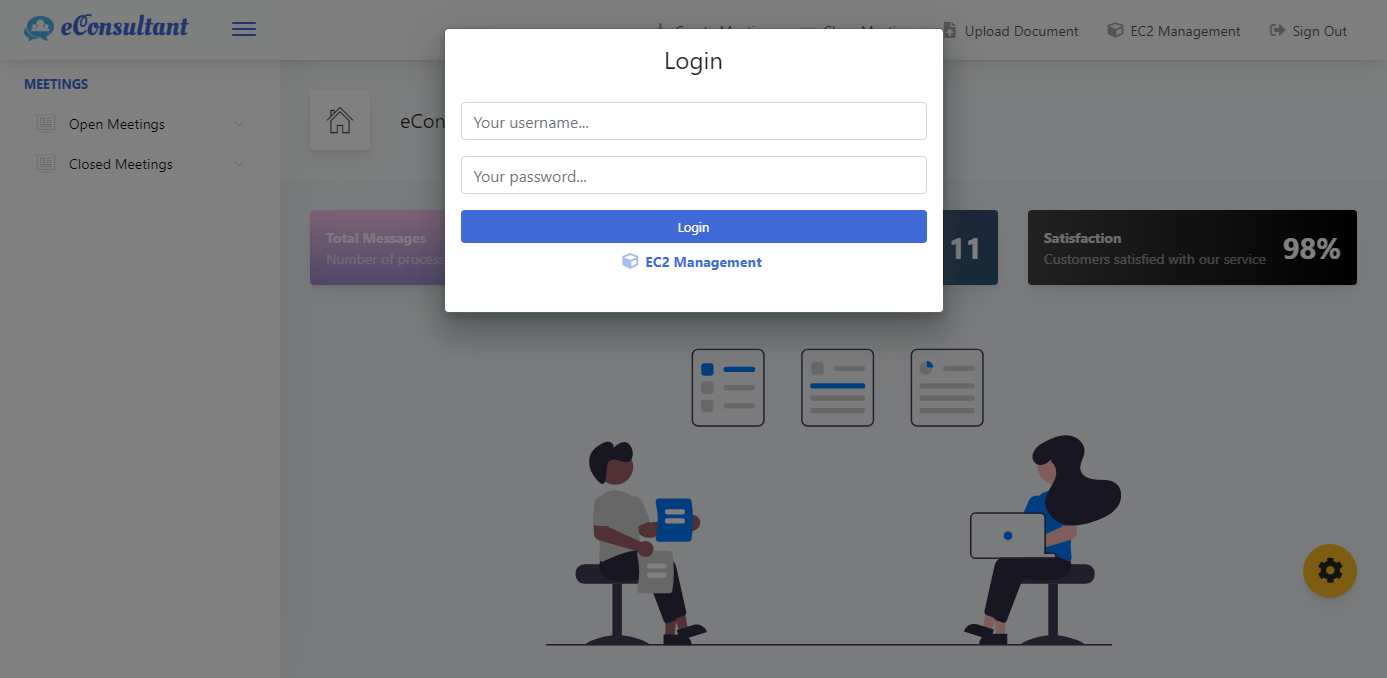
\includegraphics[scale=0.295]{implementation/login.jpg}
  \caption{Login modal}
  \label{fig:login}
\end{figure}

{\large 
Figure \ref{fig:dashboard} shows the information administrator can see after logging in. Their username is displayed on the top of the page, while three banners are showing the number of total messages processed by eConsultant, total number of meetings and customer satisfaction rate.\par
}

\begin{figure}[H]
  \centering
  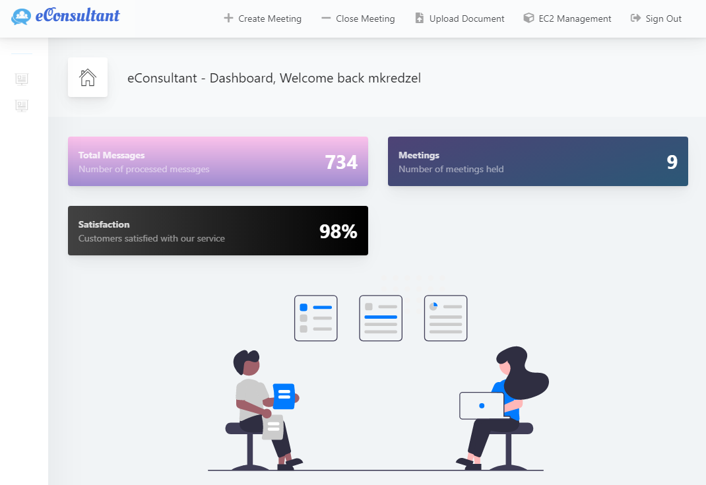
\includegraphics[scale=0.75]{charts/dashboard.png}
  \caption{Administrator dashboard}
  \label{fig:dashboard}
\end{figure}

{\large 
Navigation bar allows administrator to perform several tasks. Figures \ref{fig:createMeeting}, \ref{fig:closeMeeting} and \ref{fig:uploadDocument} present creating new meeting, closing existing meeting and uploading a PDF document to the specific meeting. These actions are possible thanks to Express.js server with REST API that can manipulate the data from the database. Uploading a document stores a pdf document on the server first, so it can be read, analysed by Amazon Comprehend and send to the Amazon DynamoDB.\par
}

\begin{figure}[H]
  \centering
  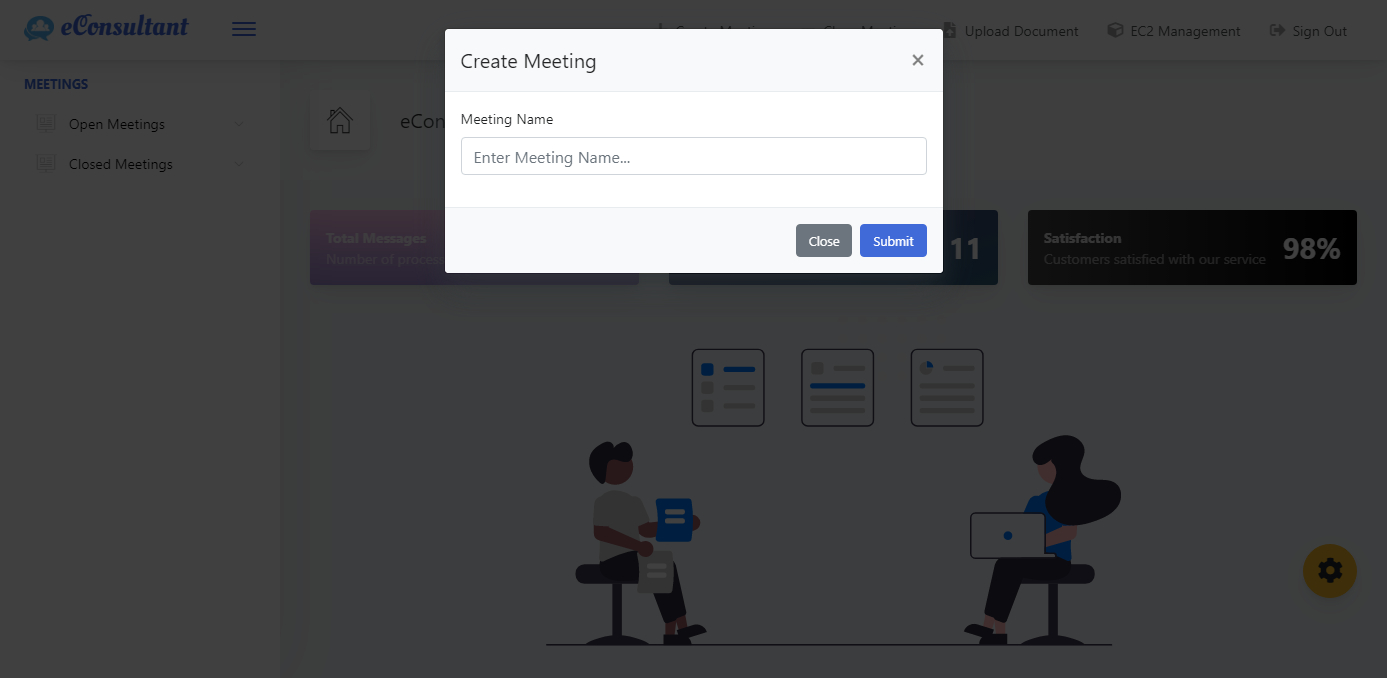
\includegraphics[scale=0.295]{implementation/createMeeting.jpg}
  \caption{Create meeting modal}
  \label{fig:createMeeting}
\end{figure}

\begin{figure}[H]
  \centering
  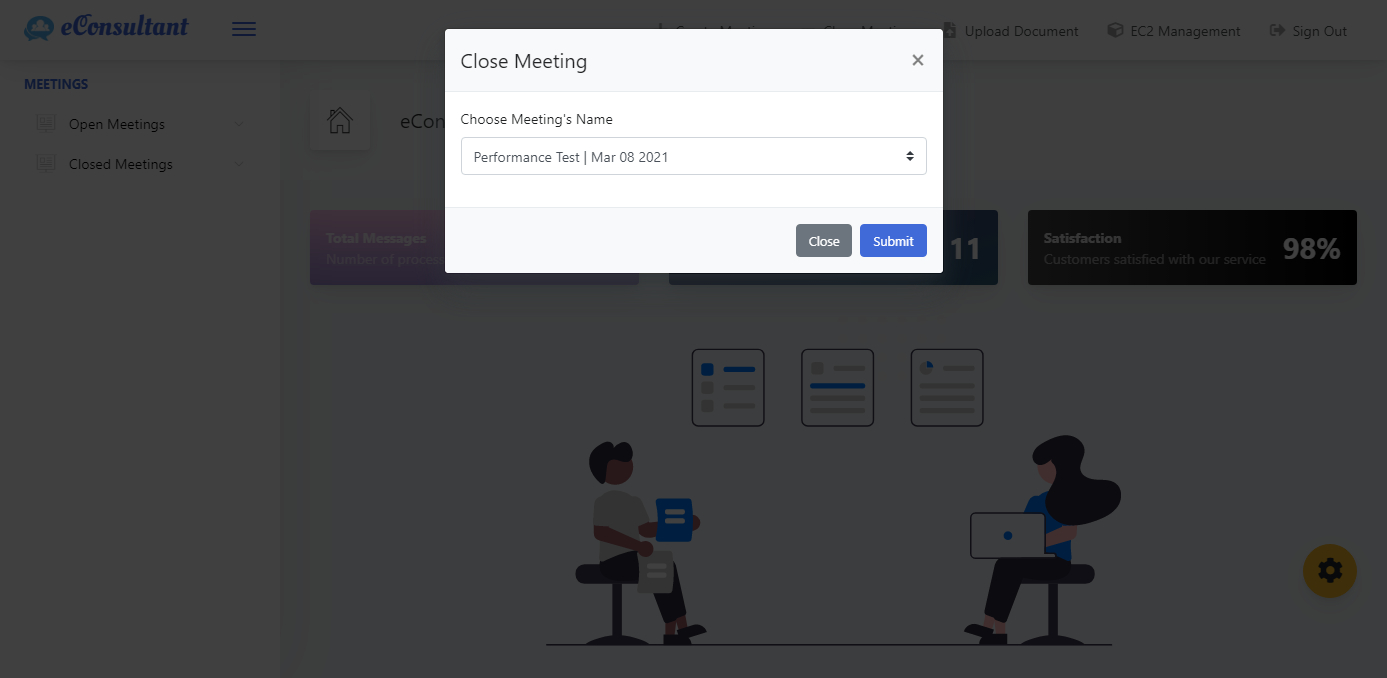
\includegraphics[scale=0.295]{implementation/closeMeeting.jpg}
  \caption{Close meeting modal}
  \label{fig:closeMeeting}
\end{figure}

\begin{figure}[H]
  \centering
  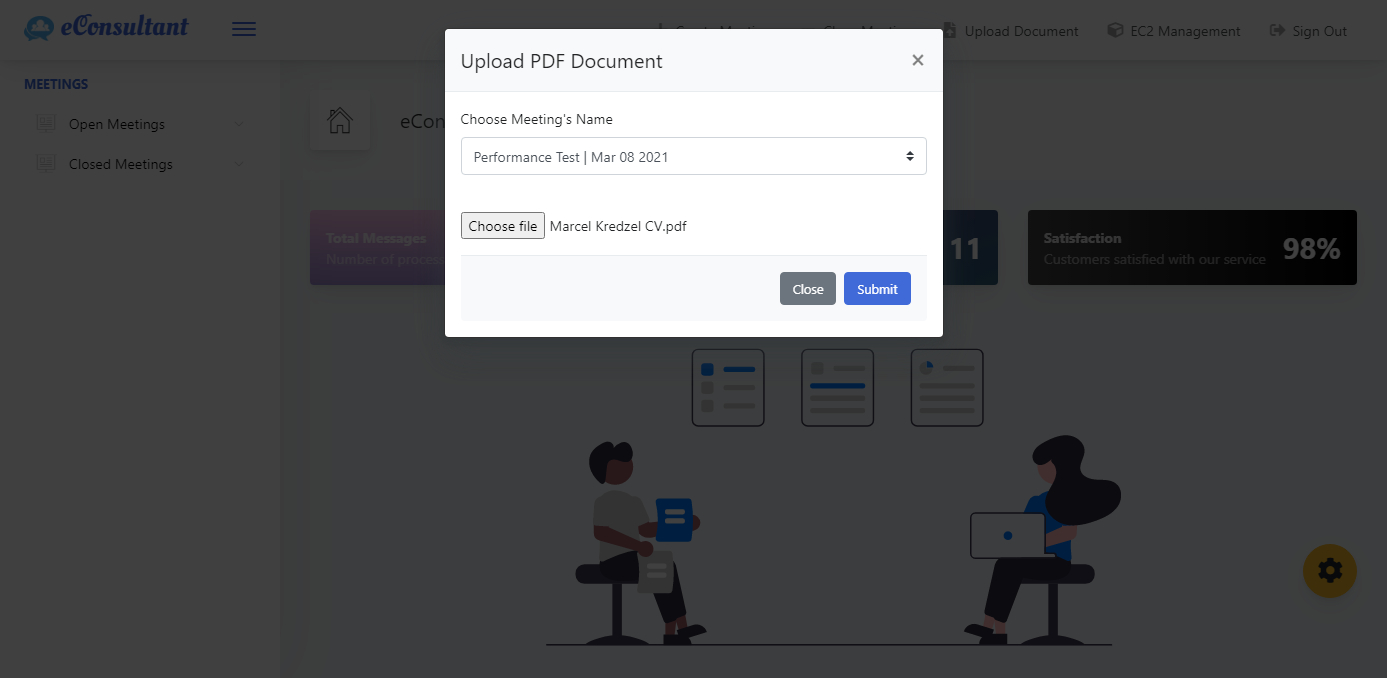
\includegraphics[scale=0.295]{implementation/uploadDocument.jpg}
  \caption{Upload document modal}
  \label{fig:uploadDocument}
\end{figure}

{\large 
Users can access data from any opened or closed meeting by selecting it from the list of meetings. The meeting's name is displayed on the top of the page next to the filter option. Filter allows to choose one or all users' data to be displayed in the tabs. The first tab is the ``Messages'' tab shown in figure \ref{fig:uploadDocument}. It contains five components of which all are scrollable, it means that they do not expand visually of the specified height.\par
}

\begin{figure}[H]
  \centering
  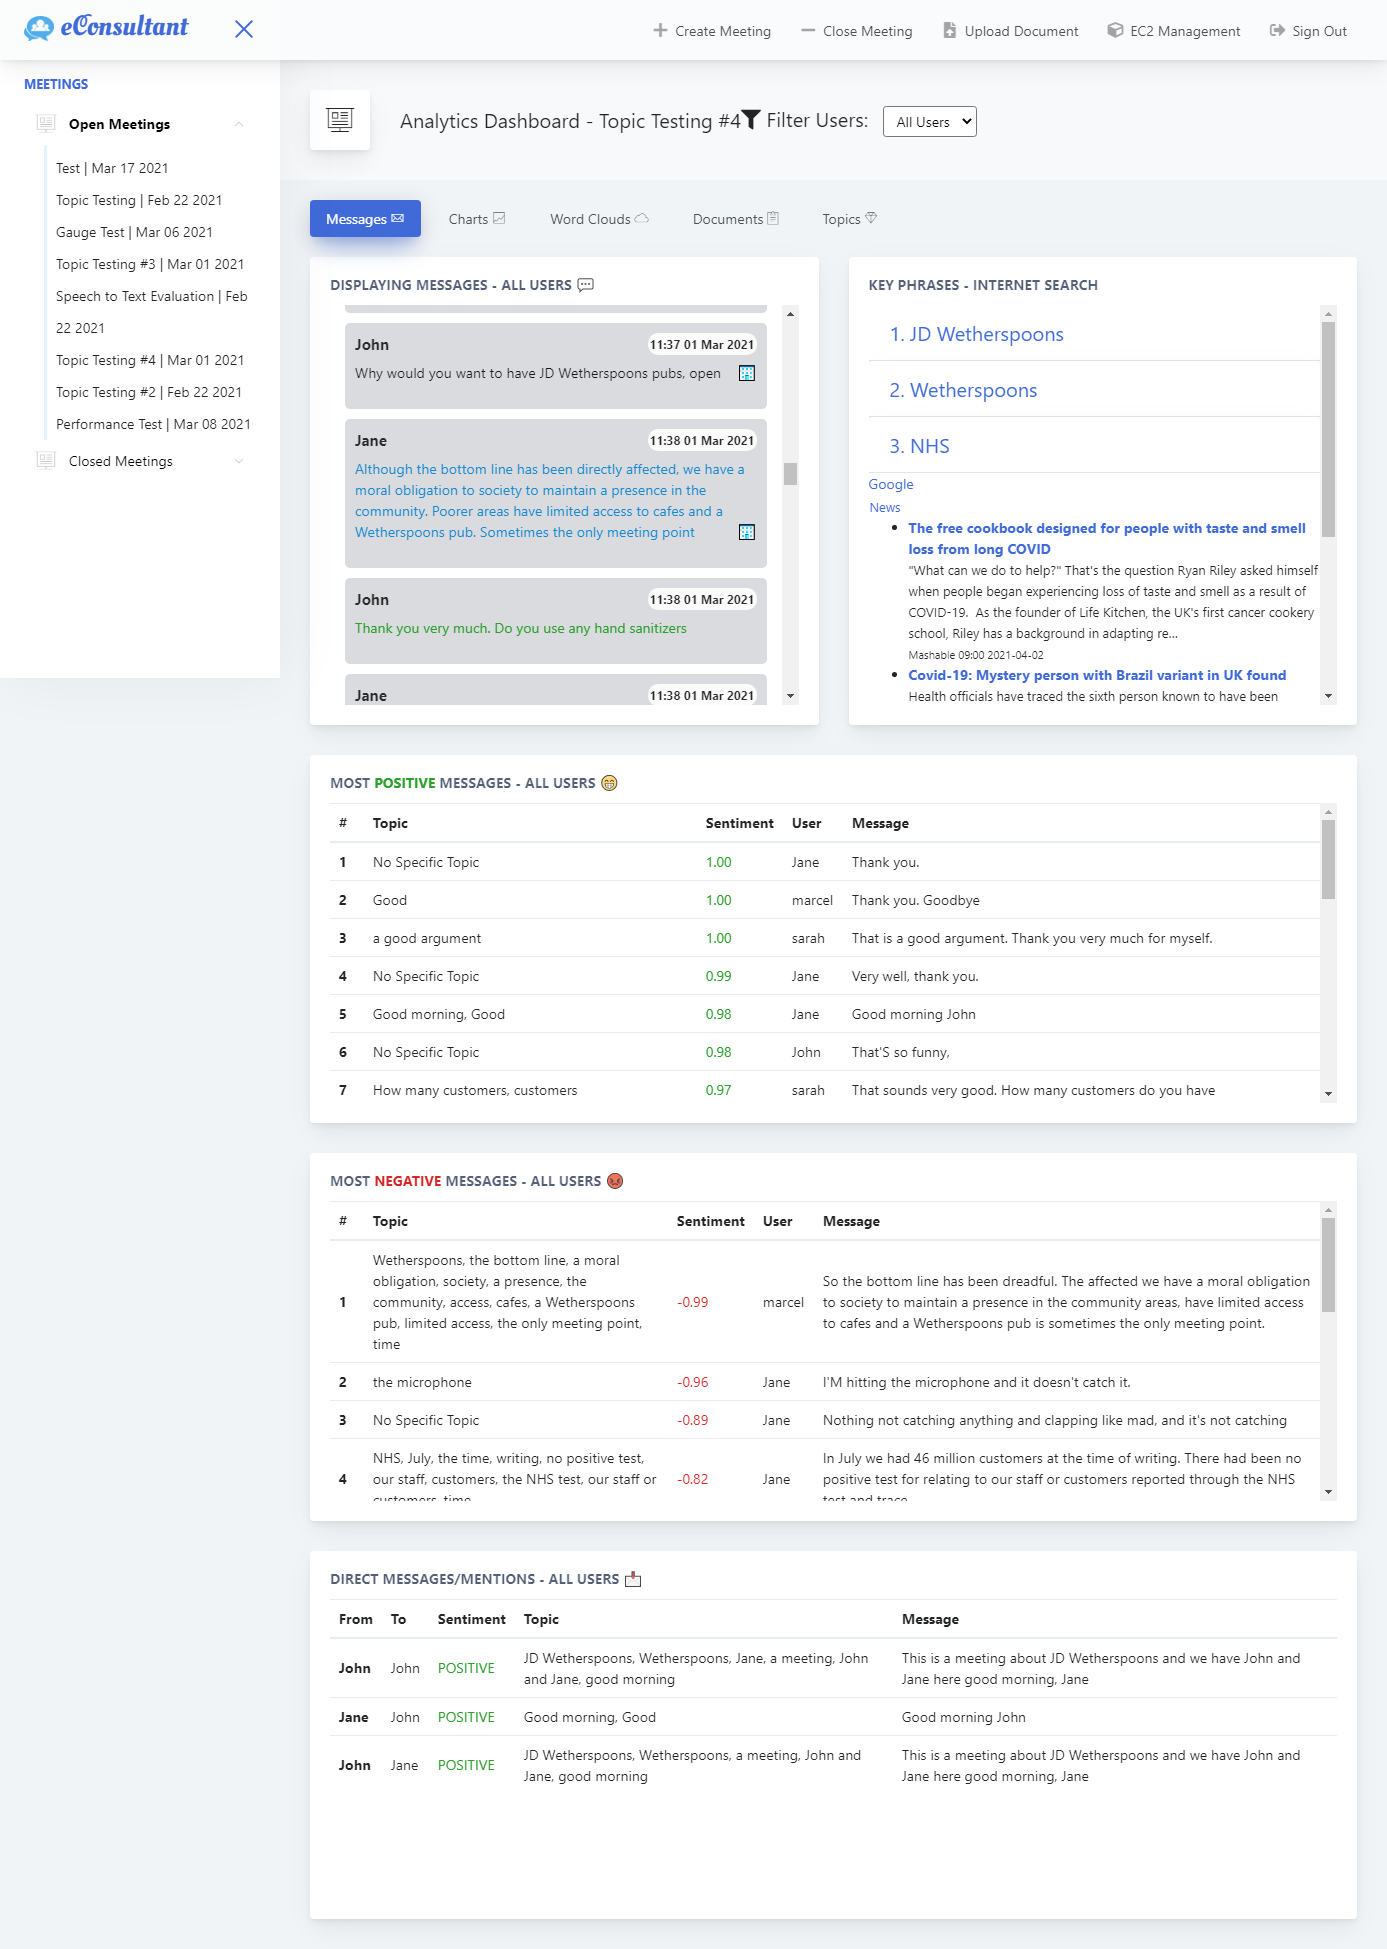
\includegraphics[scale=0.29]{implementation/messagesTab.jpg}
  \caption{Messages tab}
  \label{fig:messagesTab}
\end{figure}

{\large ``Displaying messages'' show the messages spoken in the meeting. Each message has its own sender and the time. Sentiment analysis is being applied and determined sentiment is presented as follow:  green text states positive sentiment, red text states negative sentiment, blue text states mixed sentiment and grey text states neutral sentiment. There are also emojis that show entities in the message. Recognizable entities are people, dates, locations and organizations. These entities are also represented in ``Key phrases - internet search'' component which is using Cheerio web scraper to gather some data from Wikipedia, while news are accessed through News API.\par
}

\vspace{10pt}
\begin{figure}[H]
\centering
\begin{minipage}{.5\textwidth}
  \centering
  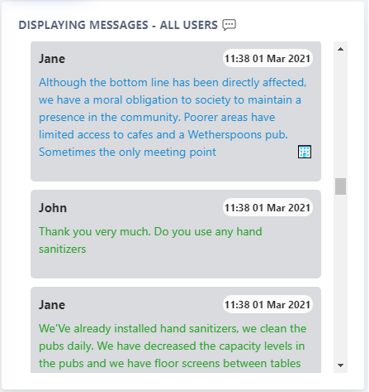
\includegraphics[width=1\linewidth]{charts/messages.png}
  \caption{``Displaying messages'' component}
  \label{fig:messages}
\end{minipage}%
\begin{minipage}{.5\textwidth}
  \centering
  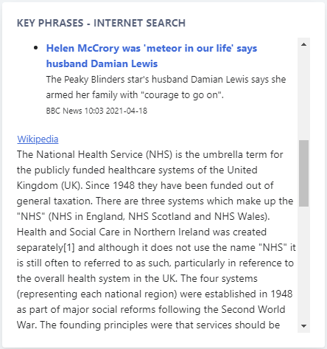
\includegraphics[width=1\linewidth]{charts/internetsearch.png}
  \caption{``Internet search'' component}
  \label{fig:internetsearch}
\end{minipage}
\end{figure}

{\large 
The next two components are tables that display the most positive and negative messages from the meeting. They show key phrases extracted from the message by Amazon Comprehend. They also show the score of the sentiment which varies from -1 to 1 (``-'' states that the sentiment is negative). The design stays intuitive thanks to the use of colours.\par
}

\newpage

\vspace{10pt}

\begin{figure}[H]
  \centering
  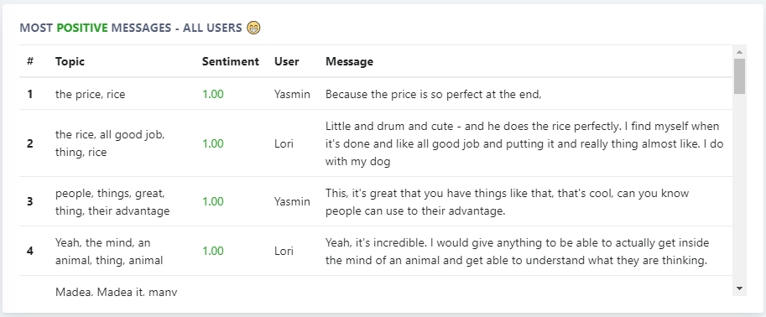
\includegraphics[scale=0.71]{charts/positive.png}
  \caption{``Most positive messages'' component}
  \label{fig:positive}
\end{figure}

\begin{figure}[H]
  \centering
  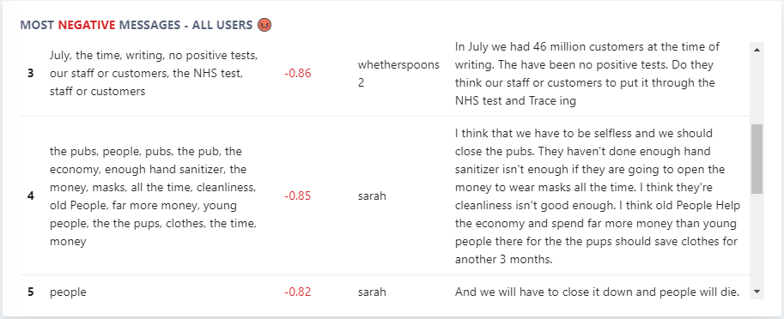
\includegraphics[scale=0.7]{charts/negative.png}
  \caption{``Most negative messages'' component}
  \label{fig:negative}
\end{figure}

{\large 
The last component in this tab is ``Direct messages/mentions'' table. It includes messages that contain the name of another user who is also a participant of the same meeting. This table is an easy way to find out if participants engaged with each other or talked about other participants. The component also topics includes the message, sentiment score, user who said the message and receiver of the message.\par
}

\begin{figure}[H]
  \centering
  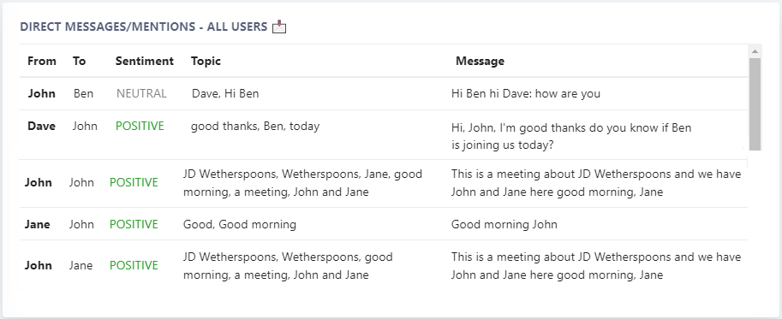
\includegraphics[scale=0.7]{charts/mentions.png}
  \caption{``Direct messages/mentions'' component}
  \label{fig:mentions}
\end{figure}

{\large 
The second tab is the ``Charts'' tab shown in figure \ref{fig:charts}. It also contains five components. All of the charts have been plotted using open source JavaScript charting libraries such as ZingChart.js, amCharts.js and Plotly.js.\par
}

\begin{figure}[H]
  \centering
  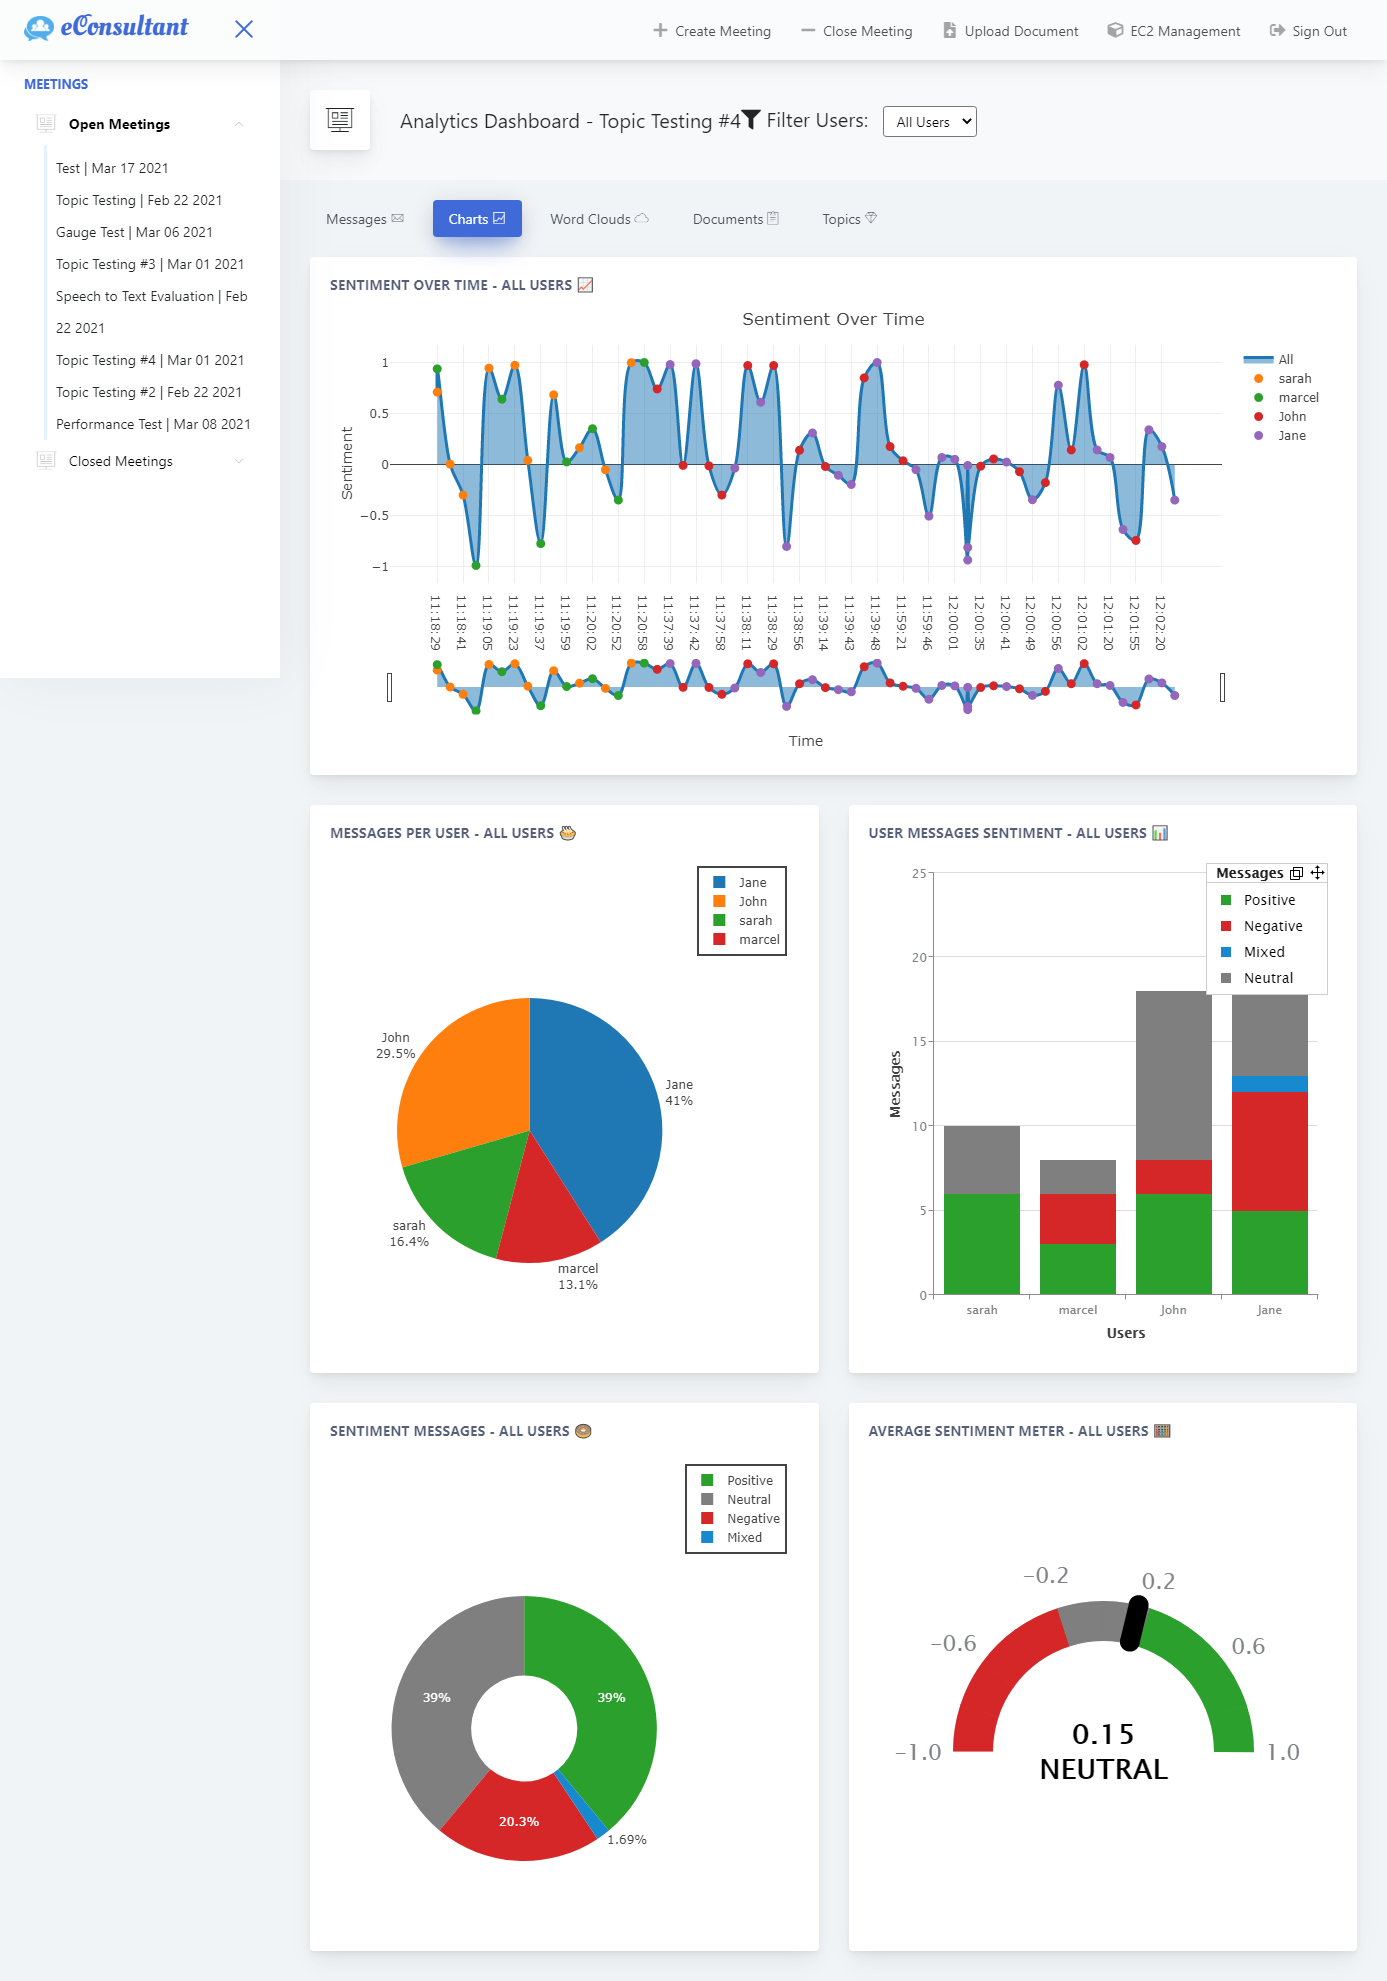
\includegraphics[scale=0.29]{implementation/charts.jpg}
  \caption{Charts tab}
  \label{fig:charts}
\end{figure}

{\large 
``Sentiment over time'' shows the filled line chart. This plot helps in understanding whether the meeting started and ended in the particular sentiment or whether there was any drastic sentiment change during the meeting. Markers are colour-labeled and they represent messages said by different users. The legend displays user names, so it is easy to locate messages of a specific user. The exact message can be seen on hover of the specific marker. There is also a slider in the bottom to filter the time range of the sent messages.\par
}

\vspace{10pt}
\begin{figure}[H]
  \centering
  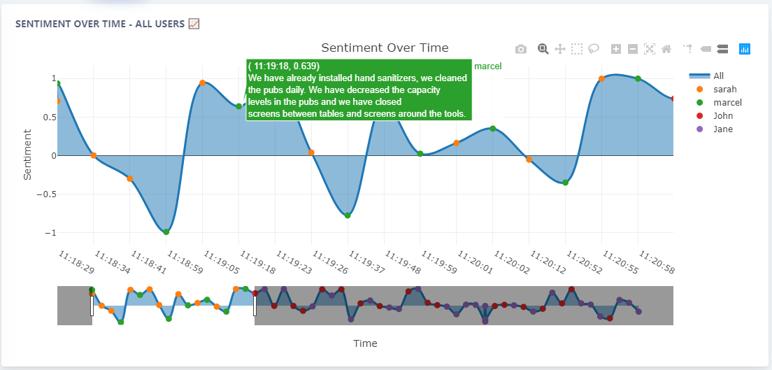
\includegraphics[scale=0.72]{charts/sentimentovertime.png}
  \caption{``Sentiment over time'' line chart}
  \label{fig:sentimentovertime}
\end{figure}

{\large 
Figure \ref{fig:pie} shows ``Messages per user'' pie chart that is used to visualize the number of messages that belong to each user, it is available on hover of the slices. It also illustrates the comparison of the percentage of messages that have been said in the meeting. ``User messages sentiment'' bar chart displays the sentiment of the messages for each user. Messages can be positive, negative, mixed or neutral. Exact number of messages they have said is available on hover of the bars. For example you can see that Sarah has been positive from the most of her speech, while Jane threw some negativity into the meeting with the most negative messages from all the users. The bar chart is presented in figure \ref{fig:usermessagessentiment}.\par
}

\vspace{10pt}
\begin{figure}[H]
\centering
\begin{minipage}{.5\textwidth}
  \centering
  \includegraphics[width=1\linewidth]{charts/pie.png}
  \caption{``Messages per user'' pie chart}
  \label{fig:pie}
\end{minipage}%
\begin{minipage}{.5\textwidth}
  \centering
  \includegraphics[width=1\linewidth]{charts/usermessagessentiment.png}
  \caption{``User messages sentiment'' bar chart}
  \label{fig:usermessagessentiment}
\end{minipage}
\end{figure}

{\large 
``Sentiment messages'' donut chart shows an overview of the sentiment throughout the whole meeting in \%, while ``Average sentiment meter'' gauge displays the mean of the sentiment score for the whole meeting. Both charts are shown in figures \ref{fig:sentimentmessages} and \ref{fig:gauge}.\par
}

\vspace{10pt}
\begin{figure}[H]
\centering
\begin{minipage}{.5\textwidth}
  \centering
  \includegraphics[width=1\linewidth]{charts/sentimentmessages.png}
  \caption{``Sentiment messages'' donut chart}
  \label{fig:sentimentmessages}
\end{minipage}%
\begin{minipage}{.5\textwidth}
  \centering
  \includegraphics[width=1\linewidth]{charts/gauge.png}
  \caption{``Average sentiment meter'' gauge}
  \label{fig:gauge}
\end{minipage}
\end{figure}

{\large 
The third tab is the ``Word Clouds'' tab shown in figure \ref{fig:wordCloudsTab}. It displays four different word clouds such as ``Key phrases from the conversation'', ``Most common words from the conversation'', ``Most common words from positive messages'' and ``Most common words from negative messages''. Words' size depends on the frequency of their appearance in the meeting. Word clouds have all been generated by using ZingChart.js JavaScript library.\par
}

\begin{figure}[H]
  \centering
  \includegraphics[scale=0.28]{implementation/wordCloudsTab.jpg}
  \caption{Word clouds tab}
  \label{fig:wordCloudsTab}
\end{figure}

{\large 
The fourth tab is the ``Documents'' tab shown in figure \ref{fig:documents}. This tab allows the administrator to choose the previously added document for its data to be visualized. It consists of four components of which three of them could have been seen in other tabs. These are word clouds and the sentiment chart. The new component gives the administrator a chance to choose the document and display its text divided into sentences, which are also analysed by Amazon Comprehend.\par 
}

\begin{figure}[H]
  \centering
  \includegraphics[scale=0.29]{implementation/documents.jpg}
  \caption{Documents tab}
  \label{fig:documents}
\end{figure}

\begin{figure}[H]
  \centering
  \includegraphics[scale=0.21]{implementation/topicsTab.jpg}
  \caption{Topics tab}
  \label{fig:topicsTab}
\end{figure}

{\large 
The fifth tab is the ``Topics'' tab.  lets users selecting multiple topics from the meeting and the documents. After selecting the topics four charts are generated.\par
}

\begin{figure}[H]
  \centering
  \includegraphics[scale=0.75]{charts/topics1.png}
  \caption{Topics drop-down menu}
  \label{fig:topics1}
\end{figure}

{\large 
 The ``Topics sentiment'' is the most advanced chart of all due to its on click triggers. It adds markers to the chart depending on the sentiment of the sentence. Once marker is clicked, dialog window of jQuery UI library pops up and displays the meeting's sentence or the document's text with the topic highlighted in yellow colour. These dialog windows are draggable and they do not close on change of the tab. The legend explains different colours and shapes. Shapes represent different sources. Circles state that a topic was used in the sentence from the meeting, while stars mean a topic was used in one of the documents. Colours represent different users or different documents. Figure \ref{fig:topics2} shows markers on hover message, while figure \ref{fig:topics3} presents dialog windows in action.\par
}

\begin{figure}[H]
  \centering
  \includegraphics[scale=0.74]{charts/topics2.png}
  \caption{Topics chart hover}
  \label{fig:topics2}
\end{figure}

\begin{figure}[H]
  \centering
  \includegraphics[scale=0.74]{charts/topics3.png}
  \caption{Dialog windows topics chart}
  \label{fig:topics3}
\end{figure}

{\large 
The next chart, ``Sankey diagram'' uses sankey diagram to visualize the sentiment and the source from which the topic comes from. Specific sentences can be found on hover of the connections. Each topic is color coded the same way it has been done in the previous chart and this way the consistency and intuitiveness still applies.\par 
}

\begin{figure}[H]
  \centering
  \includegraphics[scale=0.76]{charts/topics4.png}
  \caption{Sankey diagram}
  \label{fig:topics4}
\end{figure}

{\large
The third topics chart, ``Force directed graph'' uses force directed graph to show relation between messages' source. Thanks to this chart, it is possible to see if there is connection between some users, documents or users and documents. Big circles represent topics. For example figure \ref{fig:topics5} shows that three people were talking about pubs: Jane, Sarah and Marcel.\par 
}

\begin{figure}[H]
  \centering
  \includegraphics[scale=0.82]{charts/topics5.png}
  \caption{Force directed graph}
  \label{fig:topics5}
\end{figure}

{\large
The last chart, ``Topics frequency over time'' uses stacked area line chart in order to visualize the frequency of topics. It clearly shows if some topics were mentioned many times, few times or not at all with emphasis on the timestamp. It can show that some topics were discussed more in the beginning of the meeting and some in the end of it. There is also a filter that gives users an option to change periods of time to 15, 30, 40 or 60 minutes.\par 
}

\begin{figure}[H]
  \centering
  \includegraphics[scale=0.82]{charts/topics6.png}
  \caption{``Topics frequency over time'' stacked area line chart}
  \label{fig:topics6}
\end{figure}

\subsection{Saving Resources}

{\large 
The only addition that was not mentioned in the design chapter before is the single page hosted on Amazon S3 bucket. This uses Amazon Cognito to authenticate the administrators and allows them to turn on and off the Amazon EC2 instance that is maintaining Node.js server, therefore it is unlikely to run out of Amazon credit before finalisation of the project. There is a Lambda function that enables or disables the instance depending on its state. Client side communicates with it through API Gateway HTTP requests. The saving resources page is shown in figures \ref{fig:ec2on}, \ref{fig:ec2pending} and \ref{fig:ec2off}.\par 
}

\vspace{20pt}

\begin{figure}[H]
  \centering
  \includegraphics[scale=0.8]{implementation/ec2on.jpg}
  \caption{EC2 instance is stopped page}
  \label{fig:ec2on}
\end{figure}

\vspace{20pt}

\begin{figure}[H]
  \centering
  \includegraphics[scale=0.8]{implementation/ec2pending.jpg}
  \caption{EC2 instance is pending page}
  \label{fig:ec2pending}
\end{figure}

\vspace{20pt}

\begin{figure}[H]
  \centering
  \includegraphics[scale=0.8]{implementation/ec2off.jpg}
  \caption{EC2 instance is running page}
  \label{fig:ec2off}
\end{figure}

\newpage
\subsection{REST API}
{\large 
Communication between the client and the database has been implemented with the creation of REST API, however it is not the only use of the API. It has also been used to make calls to other APIs such as Punctuate API and News API, scrape the Wikipedia using Cheerio web scraper, upload PDF documents and make a direct call to Amazon Comprehend for key phrase extraction and sentiment analysis.\par

\subsubsection{GET requests}

\begin{itemize}
    \item /meetingRooms
    \item /data
\end{itemize}

\subsubsection{POST requests}

\begin{itemize}
    \item /createMeeting
    \item /closeMeeting
    \item /upload
    \item /punctuate
    \item /wikiSearch
    \item /newsSearch
    \item /getKeyPhrases
\end{itemize}

Figures \ref{fig:meetingRooms} and \ref{fig:chartData} show example of data, which has been organised and sent from GET requests of this API.\par
}

\begin{figure}[H]
\centering
\begin{minipage}{.48\textwidth}
  \centering
  \includegraphics[width=1\linewidth]{implementation/meetingRooms.png}
  \caption{``meetingRooms'' - GET request}
  \label{fig:meetingRooms}
\end{minipage}
\begin{minipage}{.48\textwidth}
  \centering
  \includegraphics[width=1\linewidth]{implementation/chartData.png}
  \caption{``data'' - GET request}
  \label{fig:chartData}
\end{minipage}
\end{figure}

\subsection{Documentation}
{\large
EConsultant has been coded in JavaScript using ES6 modules what allowed generation of documentation with JSDoc. Example pages can be found in appendix \ref{fig:docs1}. User guide and deployment guide are also available in appendices \ref{page:userguide} and \ref{page:deploymentguide}.\par
}

\newpage
\section{Evaluation}
{\large 
The product has been a subject to evaluation constantly during its development. Sarah Braid, who is a consultancy expert with many years of experience in the field (former managing director of Accenture) was attending meetings with my supervisor Dr. David Gamez every two weeks. She was able to offer many insights about functional requirements. After enhancing eConsultant by new features they were later presented to Sarah for professional feedback. She is satisfied with overall results of the development and she is willing to keep professional relationship for the development of other systems she has in mind in the future.\par

Apart from meeting all the requirements, software has been tested by few methods. Firstly, the quality of HTML and CSS code have been validated using W3C service. Secondly, speech to text was tested using word error rate. Thirdly, conducted performance test allowed to see if eConsultant is capable of hosting meetings with multiple participants. Lastly, a questionnaire has been distributed to few surveyors, who were presented with a live demonstration of the system. Results of all the testing can be found in the following sections.\par
}

\subsection{HTML \& CSS Validation}
{\large 
Both HTML and CSS have been tested through their W3C validators. Figures \ref{fig:htmlvalidation} and \ref{fig:cssvalidation} demonstrate that tests were completed and no errors or warnings were found on both occasions.\par
}

\begin{figure}[H]
  \centering
  \includegraphics[scale=0.51]{implementation/html.png}
  \caption{HTML Validation}
  \label{fig:htmlvalidation}
\end{figure}

\begin{figure}[H]
  \centering
  \includegraphics[scale=0.51]{implementation/css.png}
  \caption{CSS Validation}
  \label{fig:cssvalidation}
\end{figure}

\subsection{Speech Recognition Testing}
{\large 
Speech to text has been tested using a common metric of the performance of a voice recognition system called word error rate (WER). Audio test samples have been recovered from the article mentioned in the literature review chapter \parencite{wertest}. All of the audio streams were put through eConsultant to obtain the transcript. Later on, python script that can calculate WER has been used in order to perform this test. It has been comparing two text files for substitutions, deletions and insertions. One of the files was a reference file and the second file contained the transcript received from eConsultant. The script has been found on GitHub \parencite{wer}. The results of the testing can be seen in figures \ref{fig:WERtable} and \ref{fig:WERchart}. While comparing the outcome of the testing it is clear to realise that the Google standard speech to text service has been improved. Comparing WER then and now it has decreased by almost 16\%. This score was only possible by not choosing the old, pre 2010 recordings, but the more recent ones with good quality of audio.\par
}

\vspace{20pt}
\begin{figure}[H]
  \centering
  \includegraphics[scale=1]{implementation/STT Evaluation - WER.png}
  \caption{Table of WER testing results}
  \label{fig:WERtable}
\end{figure}

\vspace{-20pt}

\begin{figure}[H]
  \centering
  \includegraphics[scale=0.78]{implementation/WERchart.png}
  \caption{Visualization of WER testing results}
  \label{fig:WERchart}
\end{figure}

\vspace{-20pt}
\subsection{Performance Test Against Requirements}
{\large 
While all of the functional requirements have been met and demonstrated in the implementation chapter, there is one particular performance test that has to be passed, otherwise the existence and need for this product would be questionable. This test has the emphasis on a requirement which states that eConsultant needs to be able to maintain stability during the meeting for dozen participants. I have written a small conditional script which is executed only in the ``Performance Test'' meeting. Every time someone would speak, the default message is being sent instead. The script is being executed at early stage so the message goes through the process any other message would go through, from punctuating API to being analysed by Amazon Comprehend and stored in Amazon DynamoDB. Figures \ref{fig:performanceTest1} and \ref{fig:performanceTest2} show that the test has been completed and the result is surprisingly good. It took three minutes to join as all different users from different browser tabs, however the messages have been sent very quick. Total of 33 messages were added to the database in the time of 30 seconds. Normally people do not speak that fast, so it shows that eConsultant is capable of hosting meetings with many participants.\par
}

\vspace{10pt}
\begin{figure}[H]
\centering
\begin{minipage}{.48\textwidth}
  \centering
  \includegraphics[width=1\linewidth]{implementation/performanceTest1.png}
  \caption{Ten users joined the meeting}
  \label{fig:performanceTest1}
\end{minipage}
\begin{minipage}{.48\textwidth}
  \centering
  \includegraphics[width=1\linewidth]{implementation/performanceTest2.png}
  \caption{Ten users talk simultaneously}
  \label{fig:performanceTest2}
\end{minipage}
\end{figure}

\subsection{Questionnaire}
{\large 
The questionnaire was created to get an overview of the usability, functionality and design of the product. The survey contains eight questions, which were asked after live demonstration of the website. Several tasks were performed during the presentation in order to receive relevant answers. There were only six, targeted computer-literates surveyors, who volunteered to take part and they prefer to stay anonymous.\par

The complete results can be found in the appendix \ref{fig:questionnaire1}, while radar chart visualizing average answers can be seen in figure \ref{fig:questionnaireChart}. Answers have been predefined using a five point Likert scale, however values have been converted from percentage to points. Answers about the usability and performance of the website have been mostly positive, however answers about using the product in the future and having the possibility of purchasing premium subscription with additional features were mixed. This feedback proves that design choices were correct and it allows to explore different ways of generating income through the product.\par
}

\begin{figure}[H]
  \centering
  \includegraphics[scale=0.76]{implementation/questionnaireChart.png}
  \caption{Visualization of average answers from questionnaire}
  \label{fig:questionnaireChart}
\end{figure}

\subsection{Feedback from Consultancy Expert}
{\large 
The former managing director of Accenture, Sarah Braid has been a huge support during all the stages of the development. She has attended every meeting I had with my supervisor to give constructive feedback on the functionality of eConsultant. We have spent several hours discussing and testing analysis of topics together with Sarah. In summary, she is happy about the development of the web application and she approved its functionality. Sarah is also interested in continuing our effective and successful cooperation in the future to enhance the software.\par
}

\newpage
\section{Conclusion}
{\large 
The goal of this project was to develop an application that can be useful for a consultant on a day-to-day basis. It explored few technologies which work well with each other, but were never really combined into one as the application that eConsultant is. The main focus was on the consultancy field and the topics it brings. This chapter goes into detail about each major technology that the system is using and summarises their technological advancements and limitations.\par
}

\subsection{Cloud Provider}
{\large 
Deploying an application to the cloud is great and comes with an extreme number of benefits. Getting to know several Amazon services and learning how to use them had a huge impact on this project. Having very little knowledge about the cloud environment when starting the development of eConsultant led to the making of some minor mistakes and poor technological choices. For example, the web application is hosted on EC2 service what makes deployment quite lengthy. Unfortunately, I did not realise I could have just used Amazon Lambda functions for the whole application instead or at least build a CI/CD pipeline using CodePipeline service.\par   
}

\subsection{Speech Recognition}
{\large 
Voice recognition is a great tool, however my choice was not the most advanced option. Web Speech API which is a free of charge browser service using Google Cloud Standard version of speech to text has one of the biggest word error rate. There were many insertions during the testing what led to poor word error rate comparing with paid services. WER could be improved by using different transcription provider. Another flaw of the service was receiving raw, non-punctuated text. Fortunately, I managed to find one open source punctuating API that has been used to resolve this problem, but it added to the complexity of the project. Unfortunately, the biggest limitation to the Web Speech API is its browser compatibility. It is only supported by Google Chrome and Microsoft Edge.\par   
}

\subsection{Sentiment Analysis}
{\large 
Amazon Comprehend sentiment analysis service is one of the best on the market right now. It is mostly correct, however it is limited when it comes to recognising irony, sarcasm and intuitiveness that humans have. One of the examples from the testing phase, ``testing negative for COVID-19'' was unfortunately determined as negative message rather than positive. Text analysis technological advancements rely on natural language processing. Machine learning improves every year, so this service will definitely improve in the future years.\par
}

\subsection{Data Visualization}
{\large 
The most important aspect of data visualization is a good understanding of the data that one wants to display. The field is very wide and offers many choices of charting libraries and paid services that can visualize data. EConsultant uses wide range of charts that are suitable for different types of data. It is possible to eliminate few of the charts that have been used and stick to one charting library to be more consistent and more clear about the design. Graphs could also be improved by doing a better job with data pre-processing to eliminate redundancies such as multiple links in force directed graph.\par
}

\subsection{Summary}
{\large 
In summary, eConsultant has a big potential of growth due to the constant improvement of the machine learning and voice recognition. Users and Sarah Braid are satisfied with eConsultant, however there is plenty of room for improvements and enhancements. For example, spending more time on designing the front-end of the website would bring more intuitiveness and ease of navigating the website. EConsultant might also have more applications than being a consultancy tool. It can analyse spoken content of any sort of meetings, so it might be used in counselling services or even in crisis and conflict assistance. Project is in hand over phase with Sarah Braid who is soon to be seeking investors to support the growth of the platform. She is planning to develop a start-up within next year. This being said, it is clear that eConsultant could convince many users in the future and become a general-purpose tool.\par
}

\pagebreak
\addcontentsline{toc}{section}{References}
\printbibliography

\newpage
\appendix
\section*{Appendices}
\addcontentsline{toc}{section}{Appendices}
\renewcommand{\thesubsection}{\Alph{subsection}}

\subsection{Requirements Specification}
\includegraphics[width=1\linewidth]{img/sarah.png}
\label{fig:sarah}

\subsection{Documentation Examples}
\includegraphics[width=1\linewidth]{img/docs1.png}
\label{fig:docs1}

\newpage
\includegraphics[width=1\linewidth]{img/docs2.png}
\label{fig:docs2}

\subsection{Questionnaire Results}
  \begin{center}
  \includegraphics[scale=0.83]{implementation/questionnaire1.png}
  \label{fig:questionnaire1}

  
  \includegraphics[scale=0.83]{implementation/questionnaire2.png}
  \label{fig:questionnaire2}
  

  \end{center}
\newpage
\subsection{User Guide}
{\large 
User guide is available from \jump{page.93}{page 93}.
}

\label{page:userguide}
    \includepdf[pages=-, landscape=true, pagecommand=\thispagestyle{lscape}]{eConsultant - user guide.pdf}
    
\subsection{Deployment Guide}
{\large 
Deployment guide is available from \jump{page.133}{page 133}.
}
\label{page:deploymentguide}
    \includepdf[pages=-, landscape=true, pagecommand=\thispagestyle{lscape}]{eConsultant - deployment guide.pdf}

\end{document}